\documentclass{article}
\usepackage[utf8]{inputenc}
\usepackage{graphicx}
\renewcommand{\contentsname}{Table des matières}

\title{Rapport du Projet Pluridisciplinaire d'Informatique Intégrative}
\author{Pierre AUGUSTE, Aurélie DEMURE, Nicolas FERNANDEZ, Manon LECUBIN}
\date{2022-2023}

\begin{document}

\begin{figure}
    \centering
    
\includegraphics[scale=0.15]{Photos/logo-universite-de-lorraine.svg_-1.png}
    \label{fig:my_label}
\end{figure}

\begin{figure}
    \centering
    
\includegraphics[scale=0.4]{Photos/tn_logo.png}
    \label{fig:my_label}
\end{figure}


\maketitle Responsables du module : Olivier FESTOR, Anne-Claire HEURTEL et Gérald OSTER

\vspace{2cm}
\begin{center}
\begin{LARGE}
\textbf{Les jardins partagés}
\end{LARGE}
\end{center}

\newpage
\tableofcontents

\newpage
\section{Introduction}
Ce rapport vise à retracer l'ensemble de notre travail dans le cadre du Projet Pluridisciplinaire d'Informatique Intégrative. Le thème de ce projet est "Les jardins partagés". Son objectif est d'appliquer nos connaissances en Gestion de projet, Base de données, Web et Algorithmie pour réaliser une application répondant à un besoin concernant cette thématique en optimisant nos ressources.

Nous avons commencé par définir ce qu'était un jardin partagé avant de faire un état de l'art pour mieux cerner l'existant et nous orienter dans notre projet.

Ici, nous allons garder la version synthétique de notre état de l'art.
\begin{center}
    \begin{tabular}{|p{2cm}|p{3cm}|p{3cm}|p{3cm}|}
    \hline
        Nom & Idée en plus & Historique & Critique \\
    \hline
        SEEED & Réseau social accessible via Facebook & Budget initial : 5000€
 Début 2021 : lancement & Peu de recul sur la fiabilité de la plateforme \\
    \hline
        LePotiron & Formulaire de mise en contact 
 Blog & 2010 : lancement
 2017 : renouveau & Manque d’anticipation \\
    \hline
        PlantCatching & Ajout des plantes et des graines & 2022 : fermeture & 2022 : fermeture \\
    \hline
        Fruiteefy & Ajout confitures et sauces & Juin 2019 : création & Valorisation des circuits courts \\
    \hline
        Leaf & Entre particuliers sur tout le terroir & Juin 2022 : création & Consommation locale non promue \\
    \hline
        Aux Arbres Citoyens & Cueillettes collectives et solidaires & Fondée en 2020 & Aucune application seulement une page Web \\
    \hline
    \end{tabular}
\end{center}



\newpage
\section{Conception et implémentation}
\subsection{Base de données}

Cinq tables ont été réalisées dans notre base de données afin de mettre en place l'application. 

\begin{figure}[h!]
    \centering
    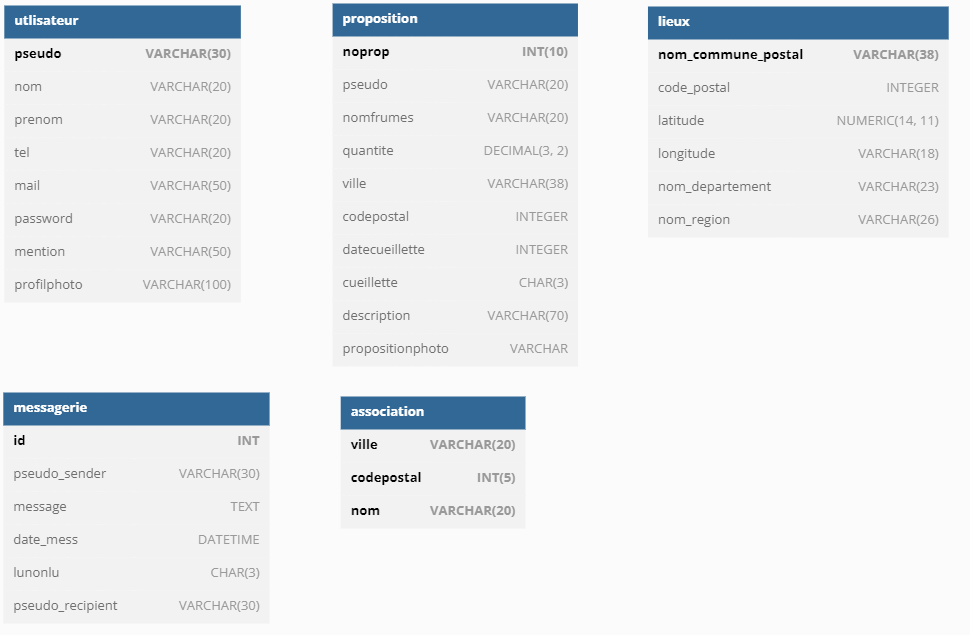
\includegraphics[width = 13cm]{Photos/BD_schema.png}
    \caption{Schéma de la base de données.}
    \label{fig:my_label}
\end{figure}


La table \textit{utilisateur} comporte les informations relatives aux utilisateurs :
\begin{itemize}
    \item Pseudo : il s’agit de la clé primaire et est donc unique. Il permet aux utilisateurs de s’identifier sur le site.
    \item Nom : contient le nom de l’utilisateur.
    \item Prénom : contient le prénom de l’utilisateur.
    \item Tel : permet l’enregistrement du numéro de téléphone de l’utilisateur.
    \item Mail : permet de même l’enregistrement de l’adresse électronique de l’utilisateur sous la bonne forme
    \item Password : enregistre le mot de passe de l’utilisateur sous forme cryptée avec l’algorithme associé.
    \item Mention : contient les informations que l’utilisateur souhaite partager sur son profil.
    \item Phofilphoto : contient l’adresse de la photo de profil de l’utilisateur.
\end{itemize}

La table \textit{proposition} enregistre les données des propositions créées par les utilisateurs :

\begin{itemize}
    \item Noprop : Il s’agit du numéro de la proposition. Cet identifiant est unique et constitue la clé primaire de la table.
    \item Pseudo : contient le pseudo du propriétaire de la proposition.
    \item Nomfrumes : contient l’information sur le fruit ou légume proposé.
    \item Quantite : permet à l’utilisateur d’indiquer la quantité de fruits/légumes proposée.
    \item Ville : indique la ville dans laquelle se trouve la proposition.
    \item Code postal : contient le code postal associé à la ville.
    \item Cueillette : contient l’information sur la cueillette (à réaliser ou non)
    \item Datecueillette : la date à laquelle les fruits ont été récoltés si la cueillette est déjà faite.
    \item Dateexpiration : la date à laquelle la proposition sera automatiquement supprimée.
    \item Description : une courte description de la proposition.
    \item Propositionphoto : contient l’adresse de la photo de la proposition.
\end{itemize}

La table \textit{lieux} comporte des informations relatives aux différents lieux que l’application peut supporter :

\begin{itemize}
    \item Nom\_commune\_postal : Il s’agit du nom de la ville. Il est élément de la clé primaire.
    \item Code\_postal : il s’agit du code postal associé à la ville. Il est également élément de la clé primaire.
    \item Latitude : contient la coordonnée de latitude correspondante à la ville.
    \item Longitude : contient la coordonnée de longitude correspondante à la ville.
    \item Nom\_departement : permet d’associer la ville avec son département.
    \item Nom\_region : permet d’associer la ville avec sa région.
\end{itemize}
	
La table \textit{association} contient les informations concernant les associations que l’application propose :

\begin{itemize}
    \item Ville : permet de connaitre la ville dans laquelle se situe l’association.
    \item Codepostal : contient le code postal de la ville.
    \item Nom : correspond à la dénomination de l’association.
\end{itemize}

Enfin, la table \textit{messagerie} qui permet la mise en place du système de communication entre les utilisateurs :

\begin{itemize}
    \item Id : il s’agit de l’identifiant du message. Il est unique et s’auto-incrémente, constituant ainsi la clé primaire de la table.
    \item Pseudo\_sender : contient le pseudonyme de l’utilisateur qui a envoyé le message.
    \item Pseudo\_recipient : contient le pseudonyme de l’utilisateur qui a reçu le message.
    \item Message : variable de texte qui enregistre le message de l’utilisateur.
    \item Date\_mess : La date et l’heure à laquelle le message a été envoyé.
    \item Lunonlu : contient l’information sur le visionnage du message 
\end{itemize}

\newpage
\subsection{Serveurs WEB}
\subsubsection{Gestion de la session}
L'utilisateur a la possibilité de se connecter sur notre application web et donc d'avoir une session. Celle-ci est gérée grâce à la fonction \textbf{Session} du module \textbf{flask\_session}. On initialise la session comme suit :
\begin{figure}[h!]
    \centering
    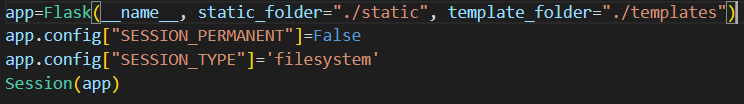
\includegraphics[width = 10cm]{Photos/Session.PNG}
    \caption{Initialisation de la session.}
    \label{fig:my_label}
\end{figure}


Ensuite, on active la session avec \textbf{session["name"]=mail}. Le mail de l'utilisateur est utilisé ici pour le nom de la session, car il définit uniquement l'utilisateur dans la base de données, et nous pouvons donc facilement récupérer ces informations pour les afficher sur l'application. La session peut se désactiver avec \textbf{session["name"]=None}.

L'état de la session (connectée ou non) va influencer l'affichage et l'accès aux différentes pages de l'application. On peut avoir accès à cet état avec \textbf{session.get("name")}.

        
\subsubsection{La barre de navigation}
Il existe deux barres de navigation différentes : une quand l'utilisateur n'est pas connecté, et une autre lorsqu'il est connecté.

Les deux barres se devait d'être facilement utilisables, ainsi,  elles sont contenues dans une balise \textbf{nav} à laquelle nous avons appliqué le CSS ci-dessous. De plus, chaque icône des barres renvoie vers une page de l'application, grâce à des balises \textbf{a}.

\begin{figure}[h!]
    \centering
    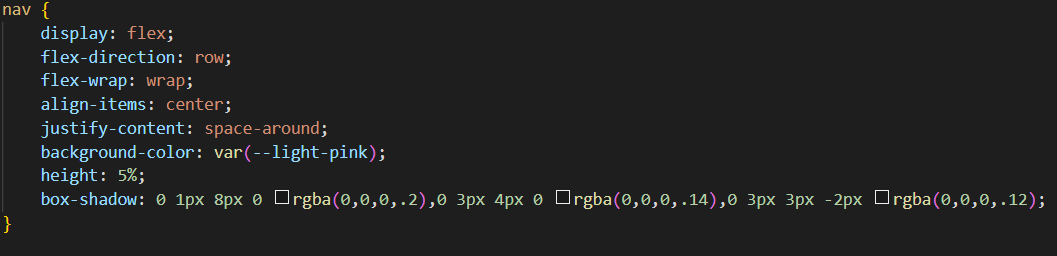
\includegraphics[width = 10cm]{Photos/CSS Bar Nav.PNG}
    \caption{Le CSS des barres de navigation.}
    \label{fig:my_label}
\end{figure}

Sur les deux barres, nous retrouvons le magnifique logo de l'application Opti'Fruit, qui renvoie vers la page d'accueil \textbf{/}. Il y a aussi un logo de groupe et un de loupe, renvoyant respectivement vers la page des associations \textbf{/associations}, et vers la page de recherche \textbf{/recherche}.

En plus de cela, la barre déconnectée possède un bouton "Inscription" et un bouton "Connexion", renvoyant respectivement vers la page d'inscription \textbf{/inscription} et celle de connexion \textbf{/connexion}. Cela nous donne la première barre de navigation :

\begin{figure}[h!]
    \centering
    \includegraphics[width = 10cm]{Photos/Barre deconnecte.PNG}
    \caption{Barre de navigation déconnectée.}
    \label{fig:my_label}
\end{figure}

Pour la barre connectée, nous retrouvons une icône pour la messagerie \textbf{/messagerie/None}, ainsi que la photo de profil et le pseudo de l'utilisateur, revoyant vers la page de profil \textbf{/profil/mail\_utilisateur}. À noter qu'à chaque apparition d'une image de profil sur l'application, on teste son existence pour l'utilisateur donné dans la base de données, avec \textbf{\{\%if profil[0]["profilphoto"]\%\}}. Si la photo n'existe pas, l'application renvoie une image de profil par défaut. Cela donne donc la deuxième barre de navigation :

\begin{figure}[h!]
    \centering
    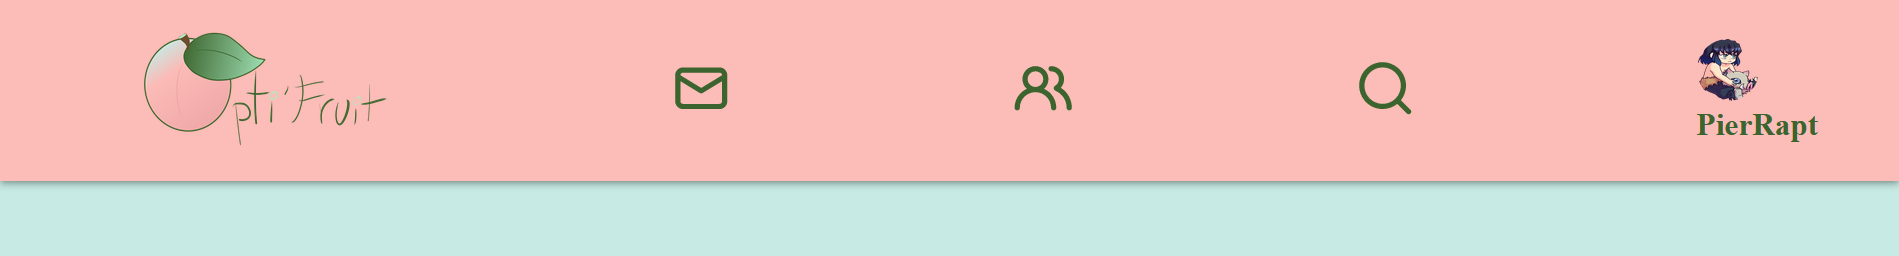
\includegraphics[width = 10cm]{Photos/Barre connecte.PNG}
    \caption{Barre de navigation connectée.}
    \label{fig:my_label}
\end{figure}

        
\subsubsection{Utilisation des layouts}
Les barres de navigation étant communes à toutes les pages de l'application, il semble pertinent d'utiliser des layouts plutôt que de recopier les barres de navigation sur chaque page. De plus, cela offre un meilleur contrôle sur quelle barre choisir. 

Ainsi, dans les fichiers html des barres de navigation, se trouvent à la fin :

\begin{figure}[h!]
    \centering
    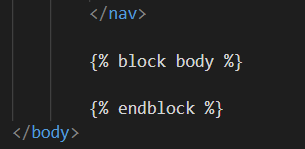
\includegraphics[width = 3cm]{Photos/block layout.PNG}
    \caption{Lignes de code indiquant que du contenu peut y être ajouté.}
    \label{fig:my_label}
\end{figure}
\vspace{5cm}
Les fichiers contenants le contenu additionnel sont sous cette forme :
\begin{figure}[h!]
    \centering
    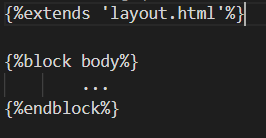
\includegraphics[width = 3cm]{Photos/extend layout.PNG}
    \caption{Syntaxe indiquant que le contenu s'imbrique dans le fichier "layout.html".}
    \label{fig:my_label}
\end{figure}

Ici, nous voulons que la barre de navigation s'adapte à l'état de la session. Pour cela, lors de la requête d'une page, on teste si la session est active ou non, comme vu précédemment. Si la session est active, c'est la barre de navigation connectée que l'on veut, sinon c'est l'autre. Le nom de la barre ainsi voulue est stocké dans une variable \textbf{navbar}, puis envoyé avec la requête du fichier html voulu. Ce dernier aura donc une en-tête de la forme : 
\begin{figure}[h!]
    \centering
    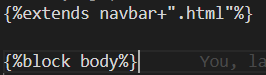
\includegraphics[width = 3cm]{Photos/extend navbar.PNG}
    \caption{En-tête des fichiers html de l'application (sauf des deux layouts).}
    \label{fig:my_label}
\end{figure}

\subsubsection{Page d'accueil}
Sur la page d'accueil se trouvent les choses les plus importantes de l'application :

Une liste synthétique des propositions existantes, avec l'image de profil et le pseudo de l'utilisateur qui a posté la proposition, la description et l'image associées.
On peut cliquer sur chacune des propositions, renvoyant sur la page de la proposition en question \textbf{/proposition/numéro\_proposition}. Si aucune proposition n'est disponible, l'application informe l'utilisateur qu'il n'y en a pas.

À côté de cette liste, il y a une image de carte renvoyant sur la page de rechercher \textbf{/recherche}, ainsi qu'un bouton "Je propose", qui renvoie vers la page d'ajout de proposition \textbf{/propose}.

\begin{figure}[h!]
    \centering
    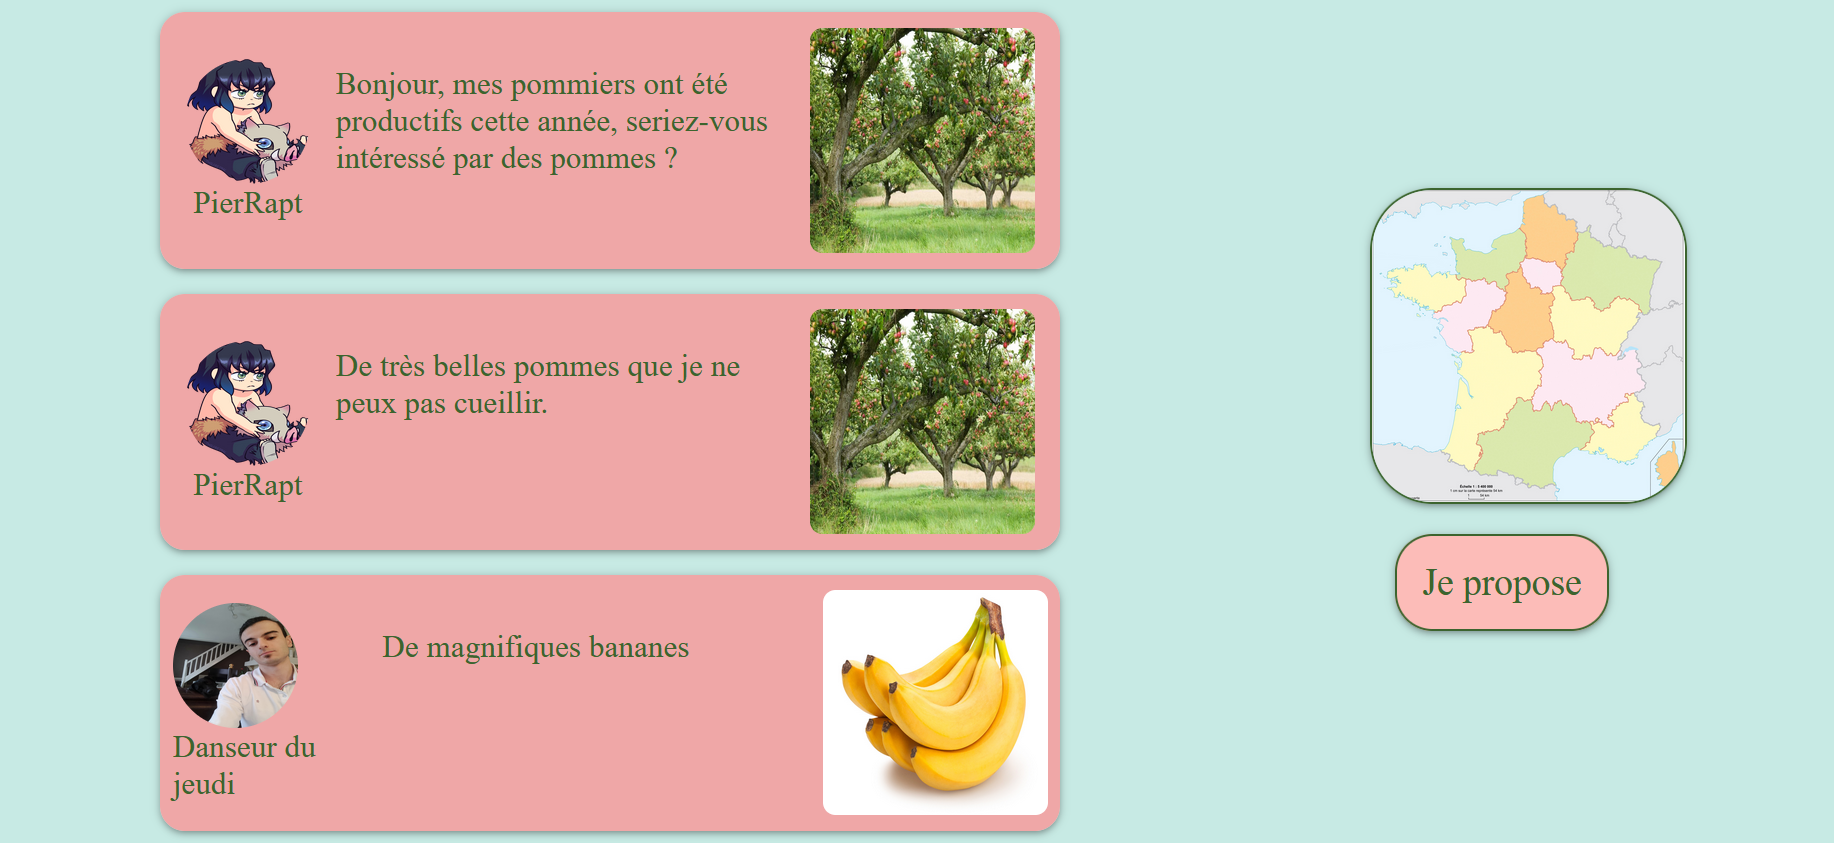
\includegraphics[width = 10cm]{Photos/home.PNG}
    \caption{La page d'accueil d'Opti'Fruit.}
    \label{fig:my_label}
\end{figure}

\vspace{5cm}
\subsubsection{Page d'ajout de proposition}

Si l'utilisateur n'est pas connecté, il est redirigé vers la page de connexion \textbf{/connexion}.

La page est composée d'un form avec plusieurs champs à remplir : Les fruits ou légumes proposés, la quantité en kg, le code postal, la ville, la description sous forme de \textbf{textarea}, une checkbox à cocher si les produits sont à cueillir, si cette dernière n'est pas cochée, une date de cueillette, une date d'expiration de la demande et un bouton pour importer une image. Enfin, un bouton "VALIDER", qui envoie les informations recueillies avec une requête POST vers \textbf{/propose}.

Lorsque la page reçoit une requête POST, elle vérifie que toutes les informations importantes sont présentes et que le code postal et la ville sont en accord avec la base de données "lieux". S'il y a un problème, l'application renvoie le form avec le message d'erreur associé au problème. Sinon, il enregistre l'image sur le serveur, et les infos dans la base de données, puis redirige vers la page de la proposition ainsi créée \textbf{/proposition/nouvelle\_proposition}.

\begin{figure}[h!]
    \centering
    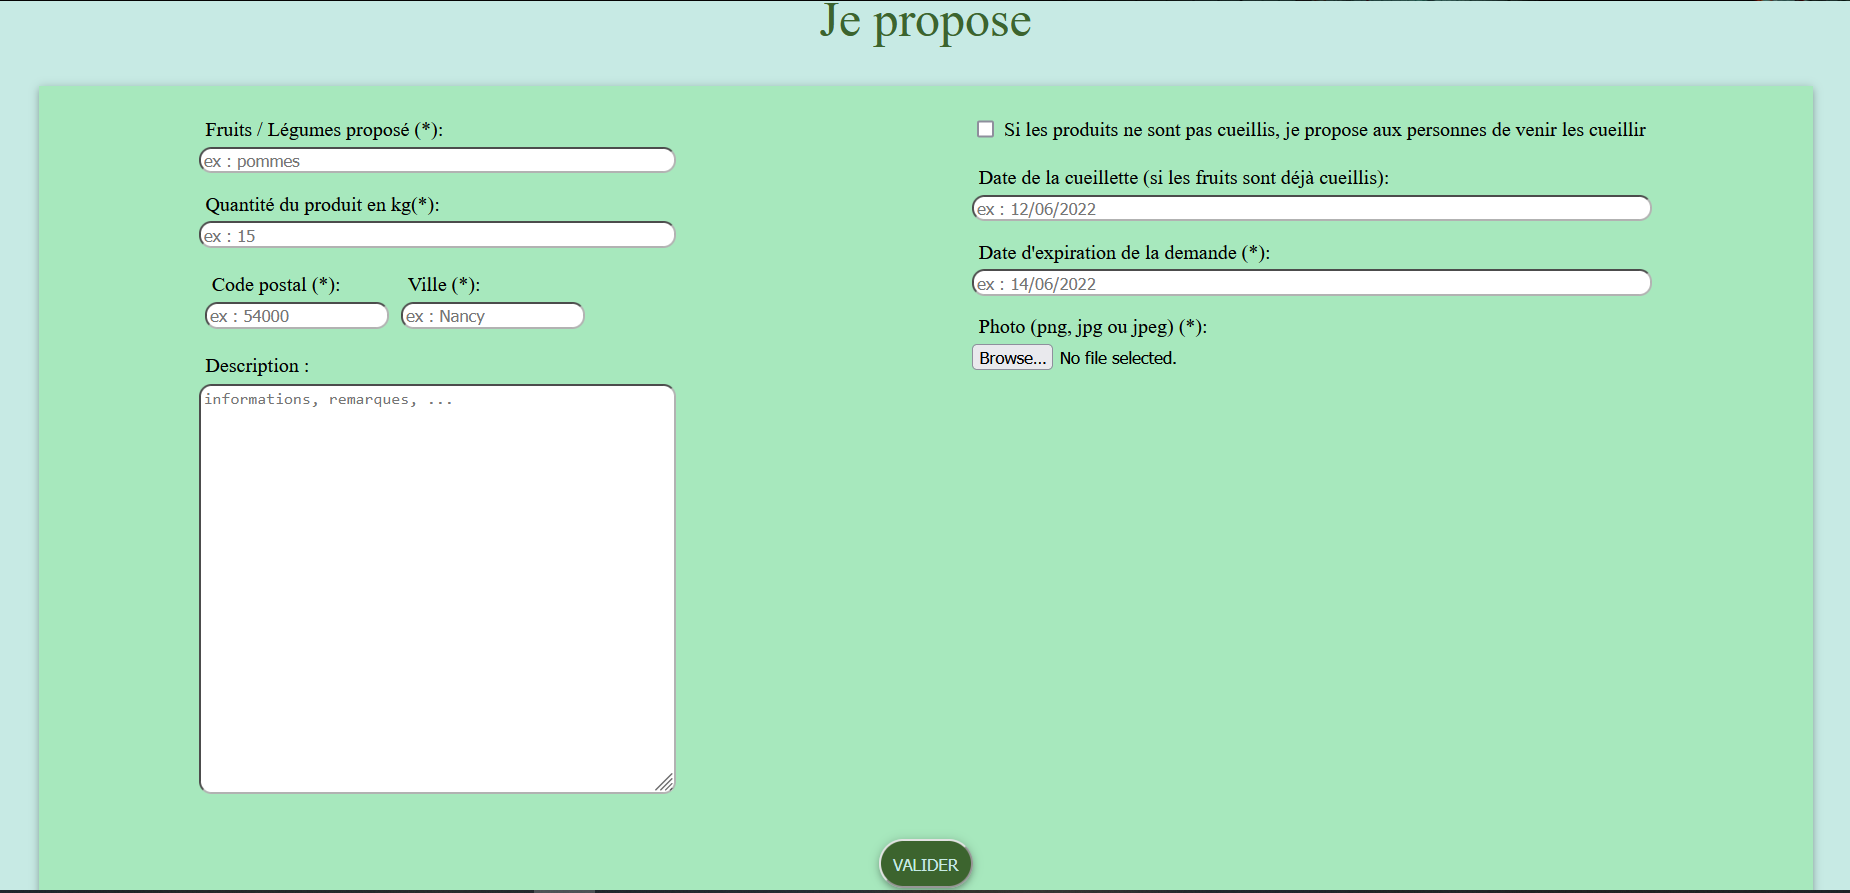
\includegraphics[width = 10cm]{Photos/ajout propose.PNG}
    \caption{La page d'ajout de proposition d'Opti'Fruit.}
    \label{fig:my_label}
\end{figure}

\subsubsection{Page d'info d'une proposition}

La page prend en paramètre un identifiant qui renvoie sur la page d'info de la proposition associée. Il y a donc une page par proposition. Sur celle-ci apparaissent toutes les info de la proposition, ainsi qu'un bouton "Home" en bas renvoyant sur la page d'accueil \textbf{/}.

De plus, si l'utilisateur est connecté, et que c'est lui qui a posté la proposition, un bouton "Supprimer la proposition" renvoie sur la page \textbf{/supprPropose/id}. Cette dernière vérifie que l'utilisateur est bien connecté (dans le cas contraire elle le renvoie sur la page d'accueil \textbf{/}), supprime la proposition avec l'identifiant \textbf{id} dans la base de données, et renvoie sur une page validant la suppression, avec un bouton "OK" validant la suppression.

\begin{figure}[h!]
    \centering
    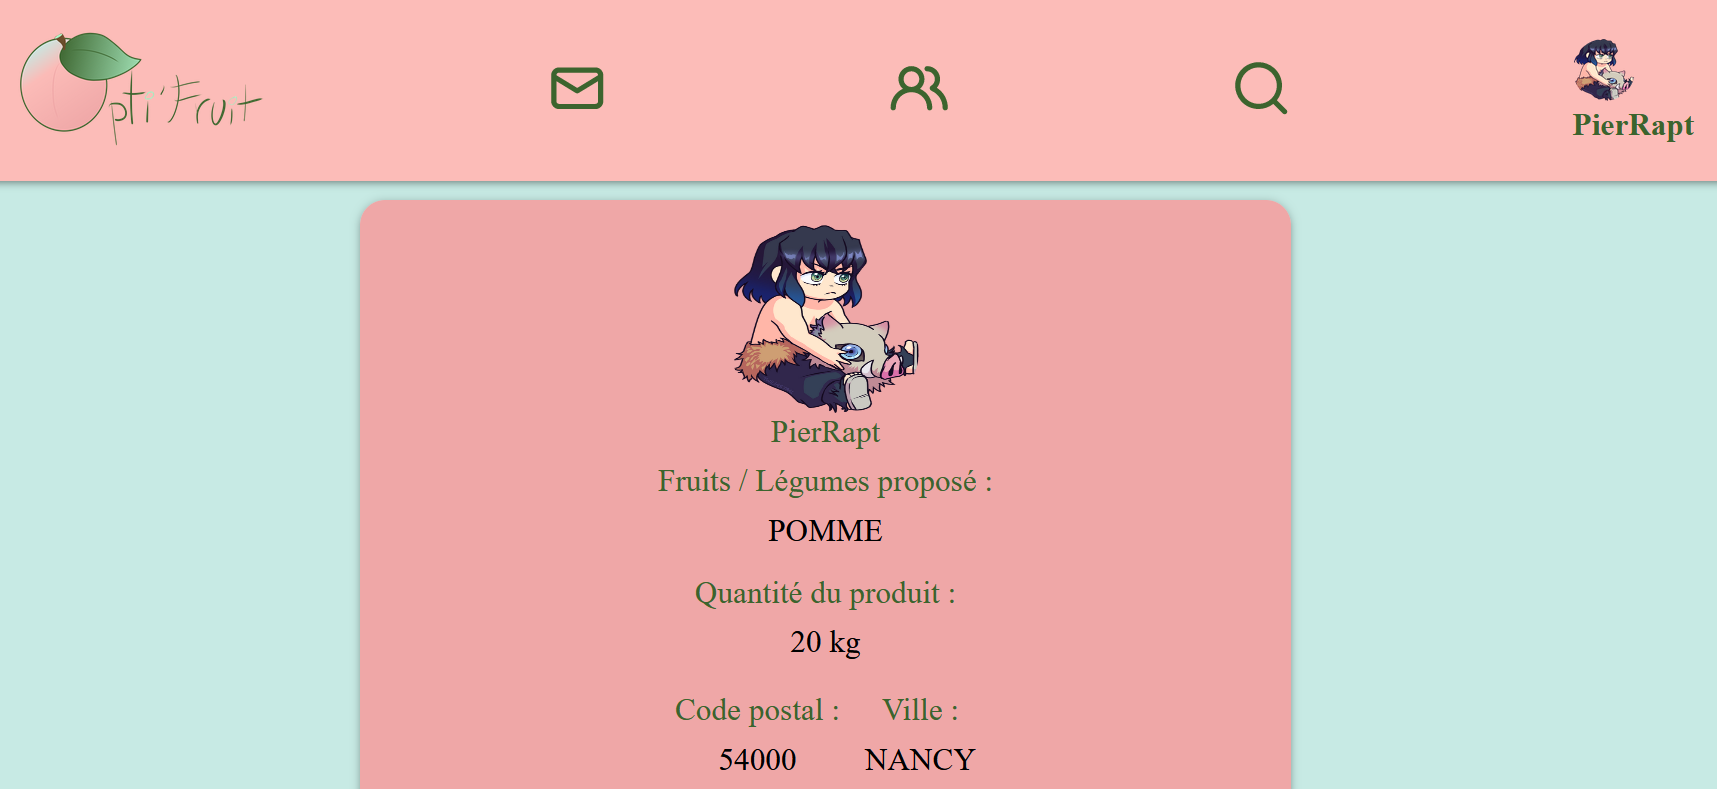
\includegraphics[width = 10cm]{Photos/proposition 1.PNG}
    \label{fig:my_label}
\end{figure}
\begin{figure}[h!]
    \centering
    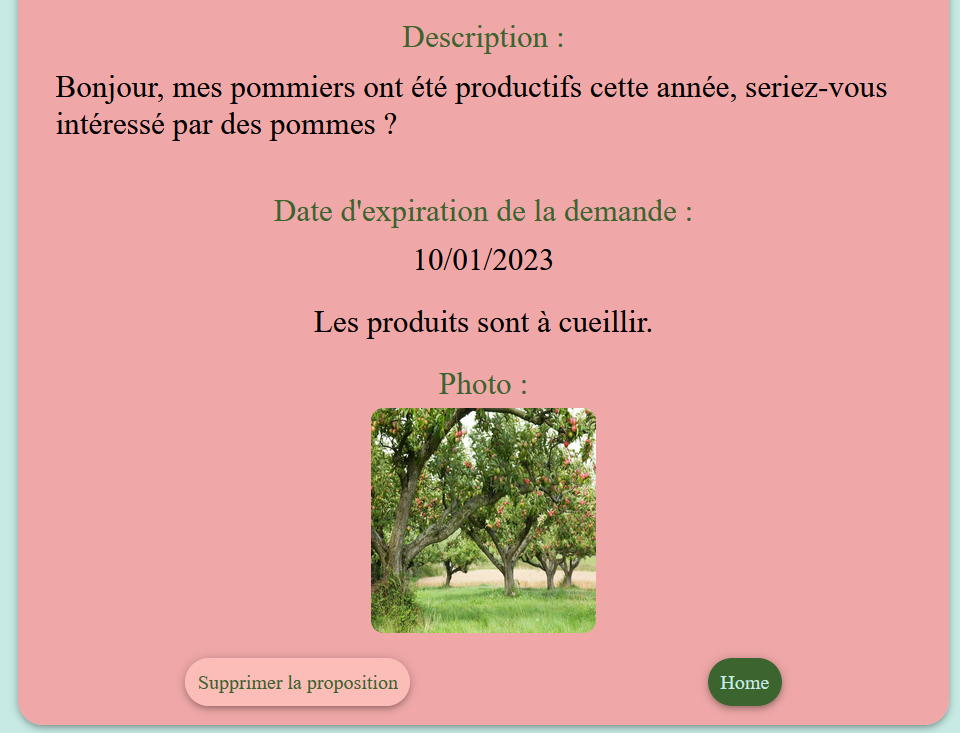
\includegraphics[width = 5cm]{Photos/proposition 2.PNG}
    \caption{La page d'information d'une proposition d'Opti'Fruit.}
    \label{fig:my_label}
\end{figure}
\vspace{2cm}
\subsubsection{Page de Messagerie}

Une fonctionnalité importante de l'application est de pouvoir échanger avec les autres utilisateurs. Si l'utilisateur n'est pas connecté, il est redirigé vers la page d'accueil \textbf{/}. Sinon, l'application récupère dans la base de données l'ensemble des utilisateurs à qui l'utilisateur connecté a envoyé un message, ou de qui il a reçu un message, triés dans l'ordre décroissant de la date du dernier message échangé. Si cette liste est vide, l'application informe l'utilisateur qu'il n'a aucune discussion.

De plus, la page prend en paramètre un pseudo d'un utilisateur existant. Si celui-ci est \textbf{None}, alors l'application ouvre la dernère discussion en cours. Si celui-ci est dans la liste des utilisateurs avec qui l'utilisateur connecté a déja échangé, la liste des messages échangés est affichée, par ordre d'envoi, accompagnée de la photo de profil et du pseudo de celui qui l'a envoyée. Le message est affiché à droite si l'auteur est l'utilisateur connecté, à gauche sinon. Tout en bas de cette liste, un champ est disponible pour écrire un message, avec un bouton "Envoyer" envoyant le message entré avec une requête POST vers \textbf{/messagerie/pseudo\_destinataire}.
Si le pseudo n'est pas dans la liste des utilisateurs avec qui l'utilisateur connecté a déjà échangé, la liste des messages est remplacée par un texte informant l'utilisateur connecté qu'il n'y a aucun message avec cet utilisateur, avec toujours le champ pour envoyer un message.

Si la page reçoit une requête POST, il insert dans la base de données le message envoyé à l'utilisateur avec qui la discussion est ouverte, et recharge la page de messagerie, affichant le nouveau message dans le flux.

\begin{figure}[h!]
    \centering
    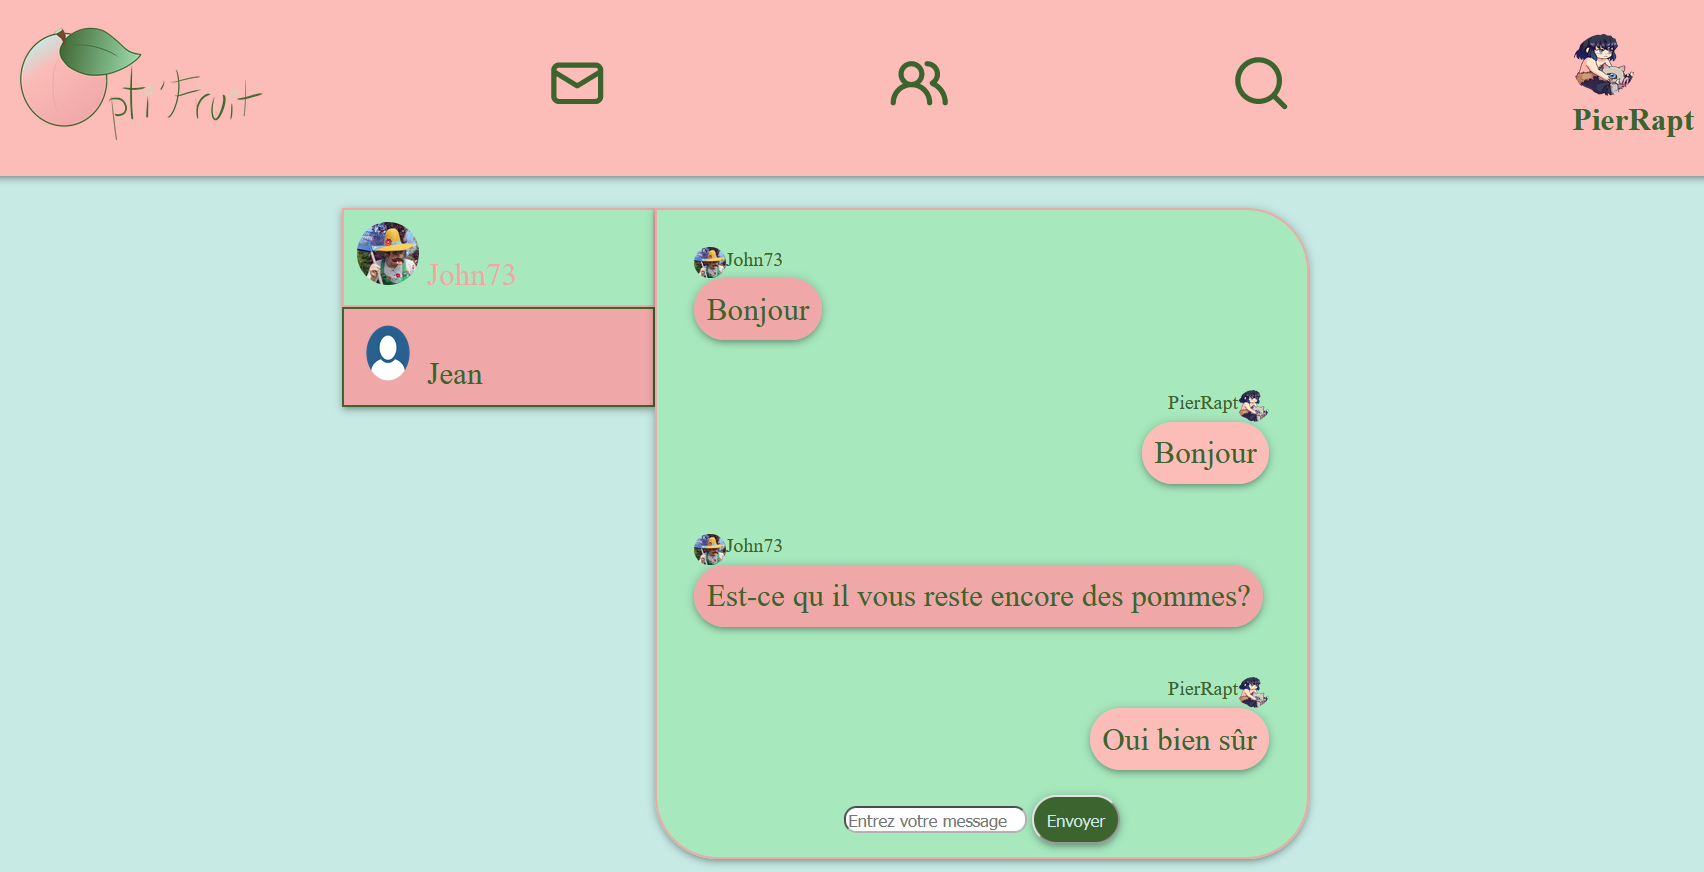
\includegraphics[width = 10cm]{Photos/messagerie.PNG}
    \caption{La page de messagerie d'Opti'Fruit.}
    \label{fig:my_label}
\end{figure}

\subsubsection{Page associations}
La page d'affichage des associations permet d'afficher toutes les associations auxquelles il est possible de donner ses fruits et légumes par ordre alphabétique des villes. Cette page permet d'afficher le nom des associations, leur code postal et leur ville après avoir récupéré ces informations dans la table \textbf{association} en utilisant une requête SQL sélectionnant la \textbf{ville}, le \textbf{codepostal} et le\textbf{nom}, avec la commande \textbf{ORDER BY} sur la \textbf{ville}. La page contient également un formulaire qui permet de rechercher les associations dans une certaine ville en utilisant dans la requête SQL la commande \textbf{LIKE} sur le nom de la ville rentrée par l'utilisateur. L'affichage se fait ensuite grâce à une grille.

\begin{figure}[h!]
    \centering
    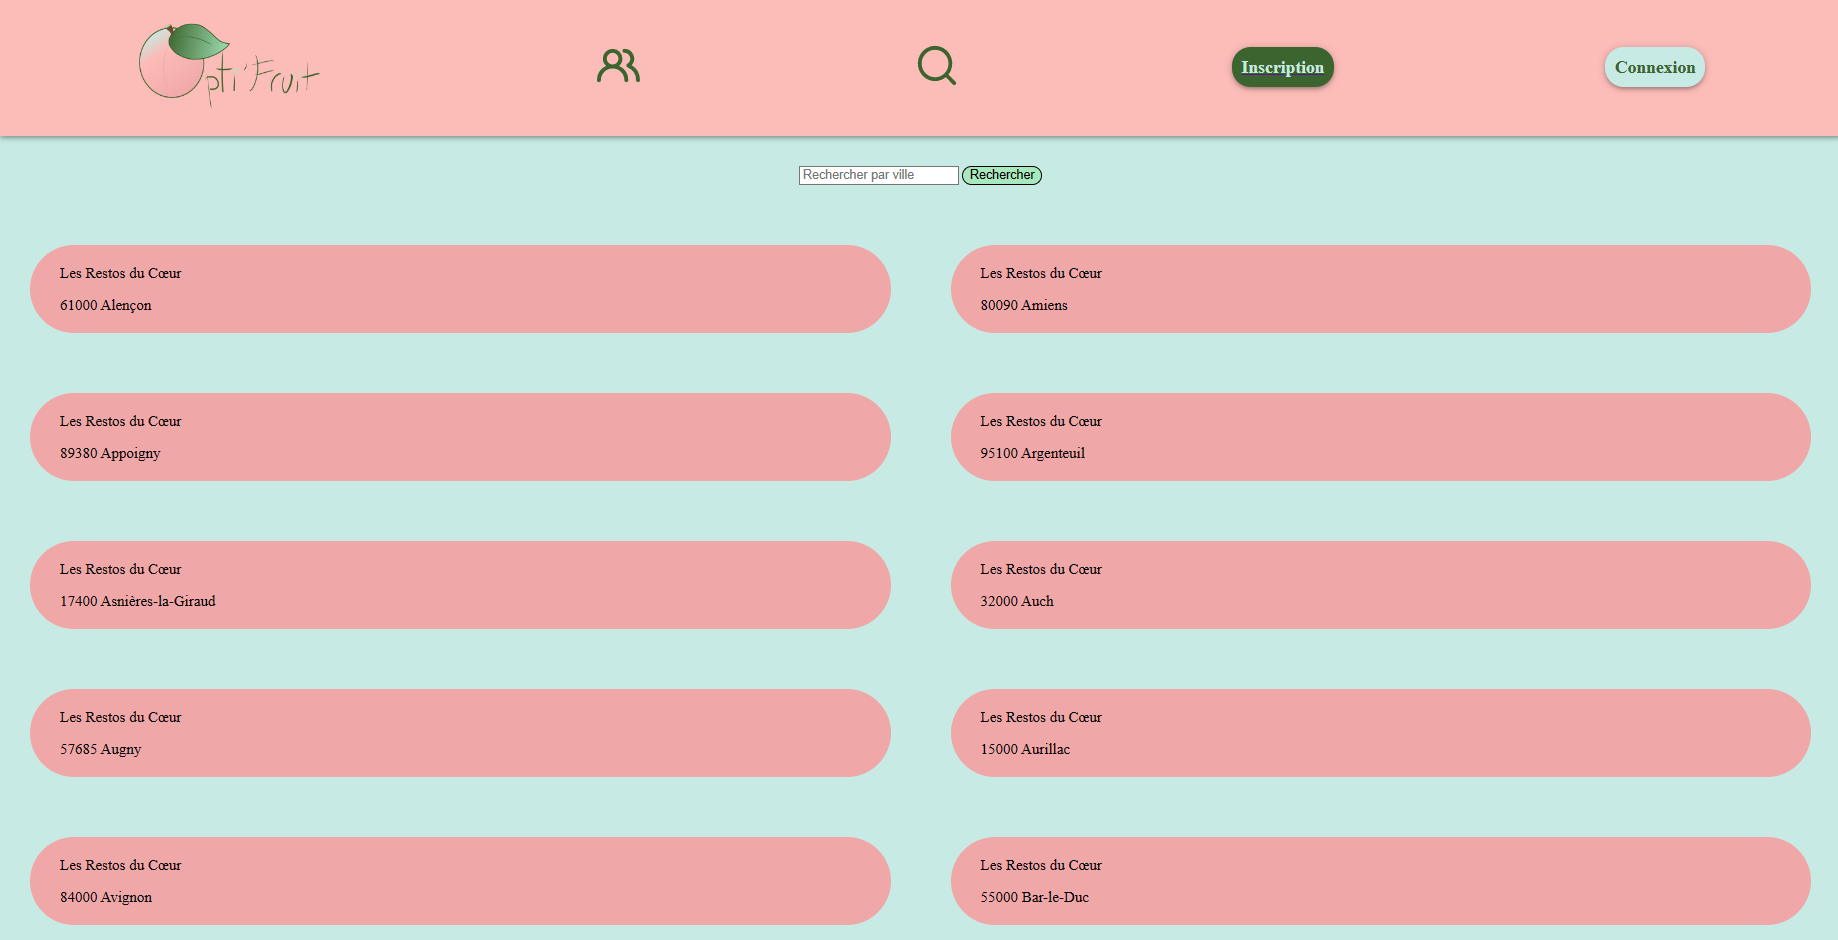
\includegraphics[width = 10cm]{Photos/page associations.PNG}
    \caption{La page des associations}
    \label{fig:my_label}
\end{figure}
\subsubsection{Page inscription}
Le principe du site étant d'avoir des utilisateurs, les nouveaux arrivants pourront s'inscrire en remplissant une série de champs. Leurs \textbf{nom}, \textbf{prénom}, \textbf{pseudo}, \textbf{numéro de téléphone}, \textbf{adressse mail} leur seront demandés ainsi qu'un \textbf{mot de passe} qu'ils devront confirmer. Ce mot de passe devra également contenir entre 8 et 20 caractères pour des raisons de complexité et sa validité sera vérifiée avant son cryptage. Le cryptage permet de ne pas enregistrer le mot de passse brut dans la base de données. Une \textbf{mention} et une \textbf{photo de profil} optionnelles seront également demandées. Sinon, aucune mention n'apparaîtra dans le profil et une photo par défaut sera ajoutée.
Une fois tous les champs remplis, un clic sur le bouton \textbf{Valider} activera la méthode \textbf{POST} de la page. Les données seront récupérées grâce à des request.
\begin{figure}[h!]
    \centering
    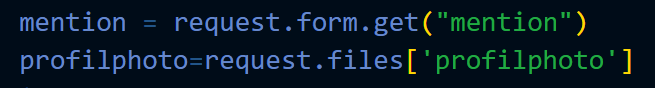
\includegraphics{Photos/request.PNG}
    \caption{Différents champs de récupération des données}
    \label{fig:my_label}
\end{figure}
\newline Si des informations obligatoires ne sont pas remplies, des \textbf{render\_templates} permettent d'afficher à l'utilisateur le message d'erreur adapté. Il faut ensuite tester les contraintes de la base de données notamment l'unicité des pseudos qui nous servent de clé primaire pour la table utilisateur. Seuls certains types de fichiers sont acceptés pour les photos grâce à un champ dans le html d'inscription.

\begin{figure}[h!]
    \centering
    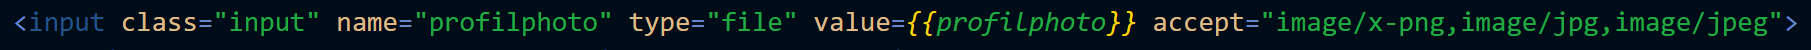
\includegraphics[width = 14cm]{Photos/Photoprofil.PNG}
    \caption{Rechercher les extensions jpg, jpeg et png}
    \label{fig:my_label}
\end{figure}
\newline
 Il est alors possible d'insérer les données de l'utilisateur dans la base de données et de le rediriger directement vers sa page de profil.

\begin{figure}[h!]
    \centering
    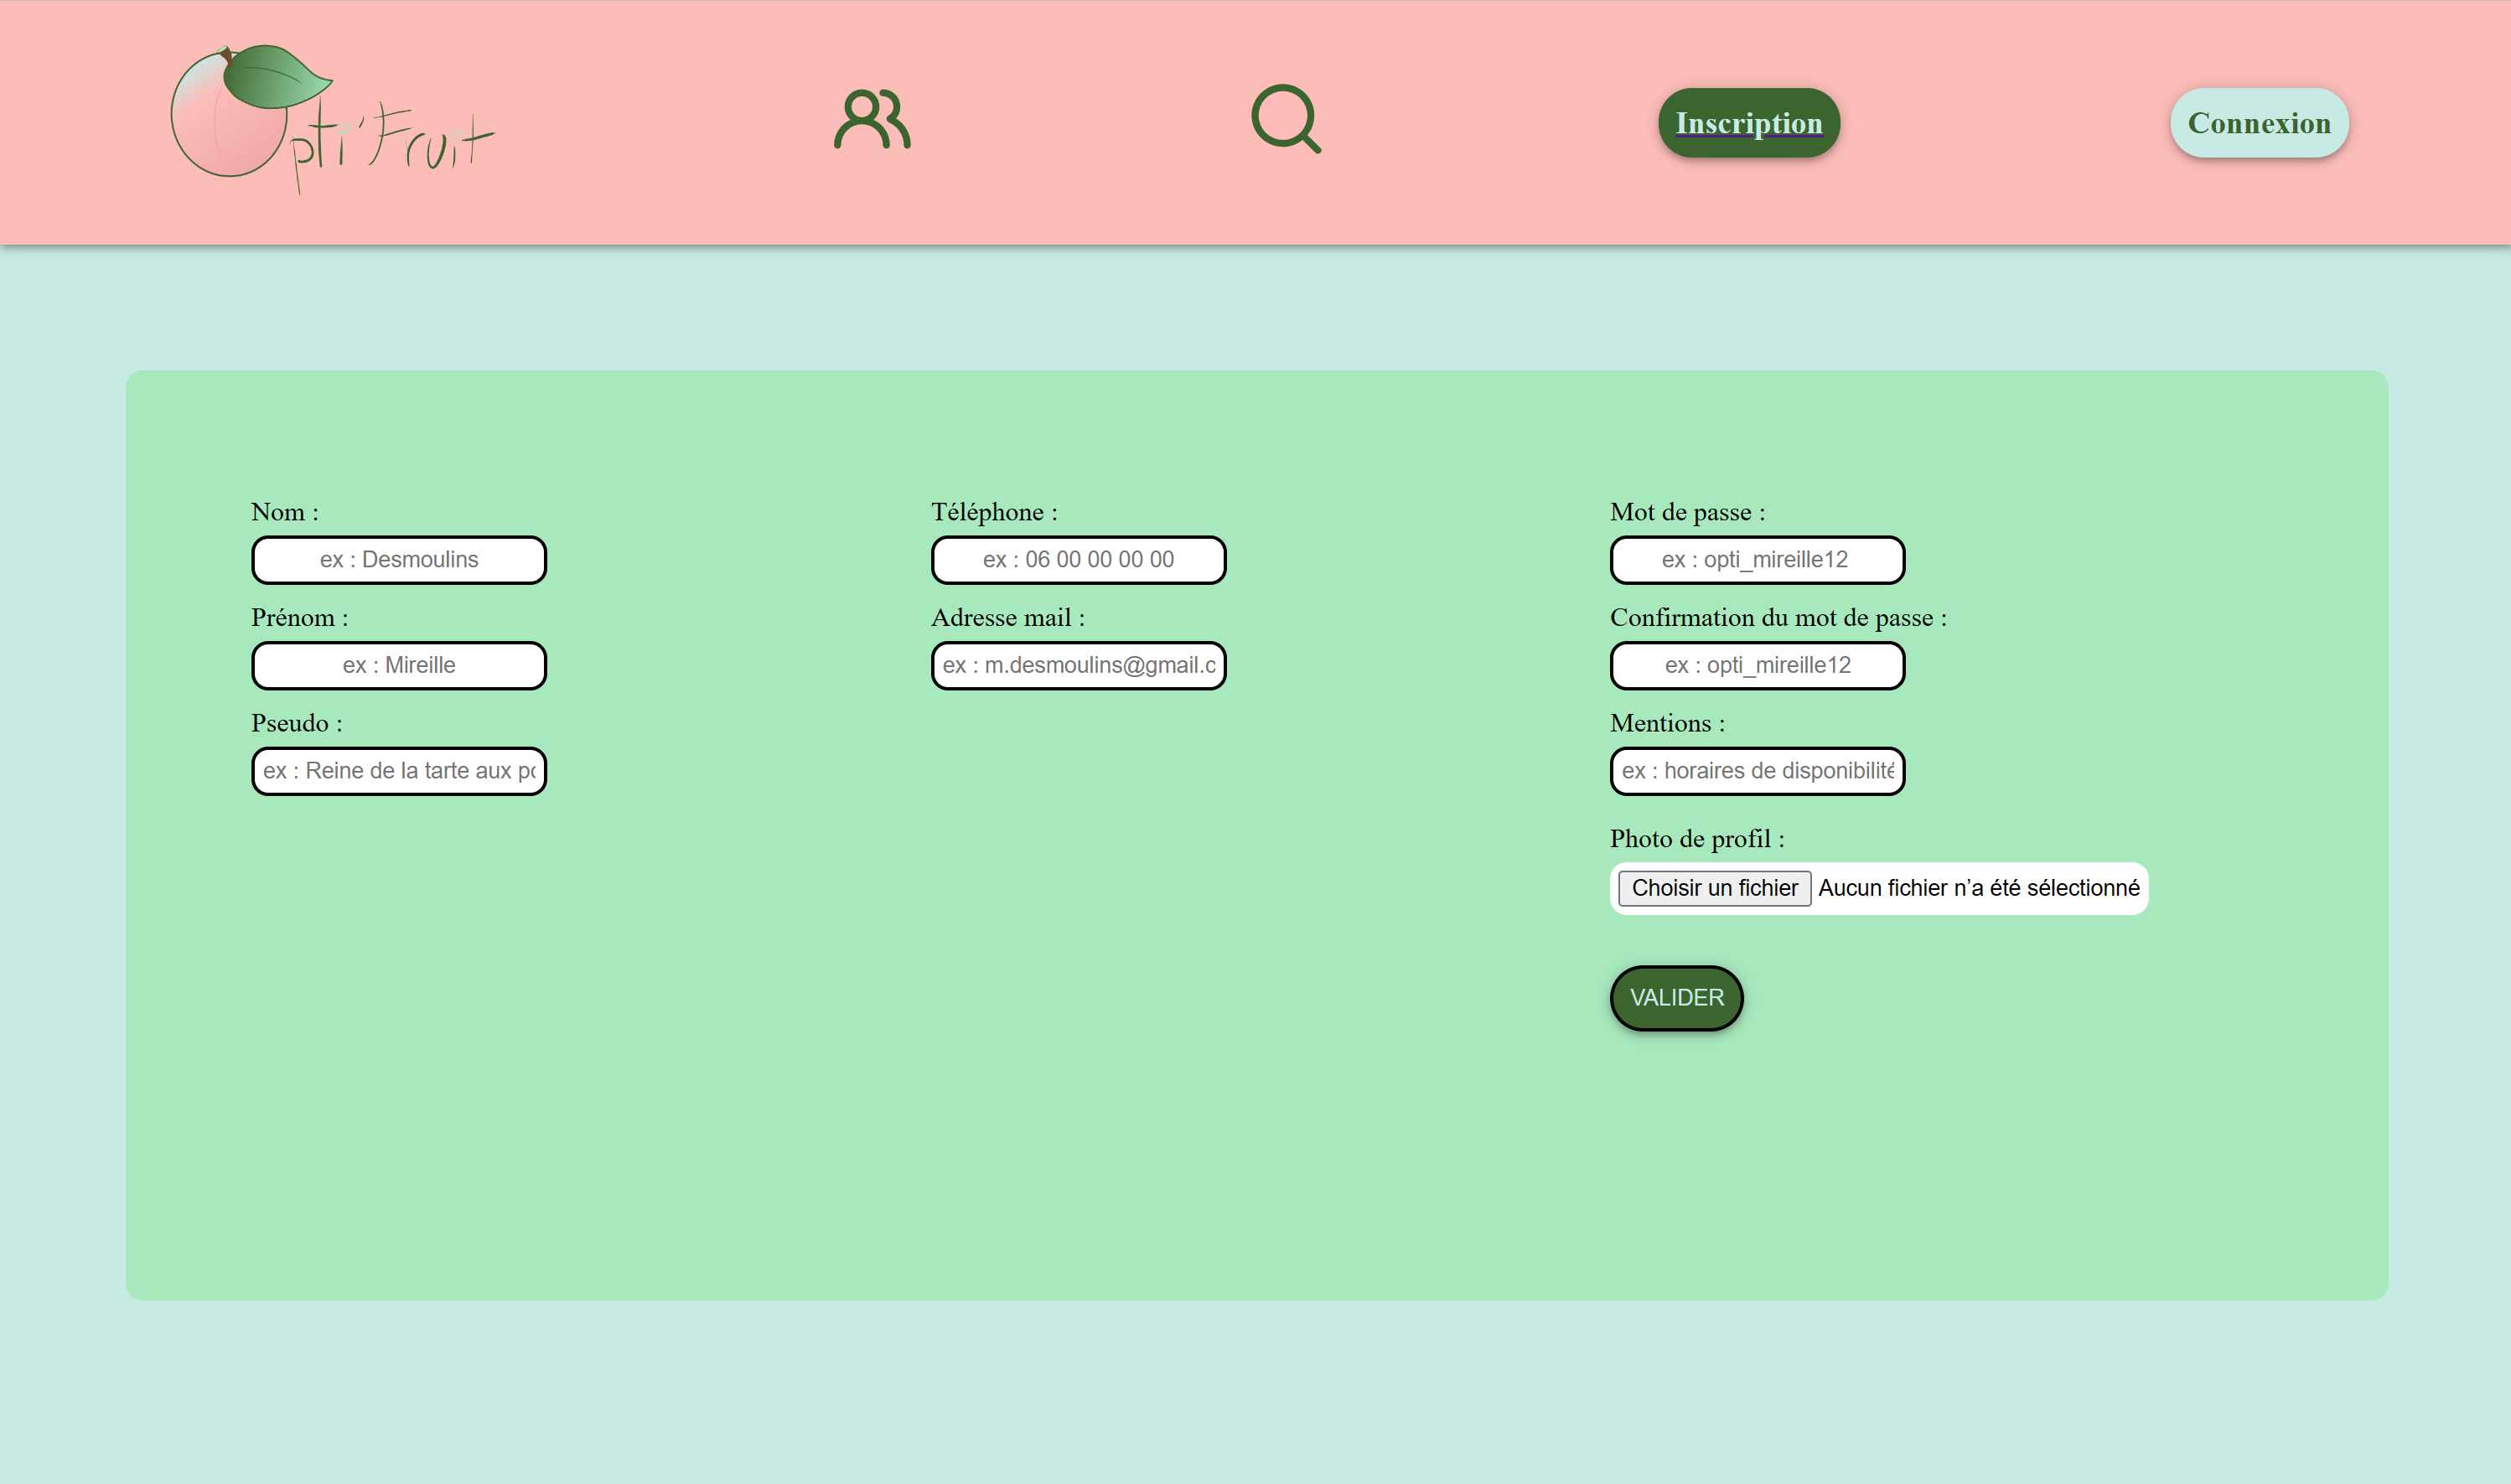
\includegraphics[width = 10cm]{Photos/Inscription.PNG}
    \caption{Page inscription à remplir}
    \label{fig:my_label}
\end{figure}

 Les champs étant étalés sur trois colonnes pour un écran d'ordinateur, il a fallu adapter le css pour des écrans de plus petites tailles tels qu'un téléphone.
\begin{figure}[h!]
    \centering
    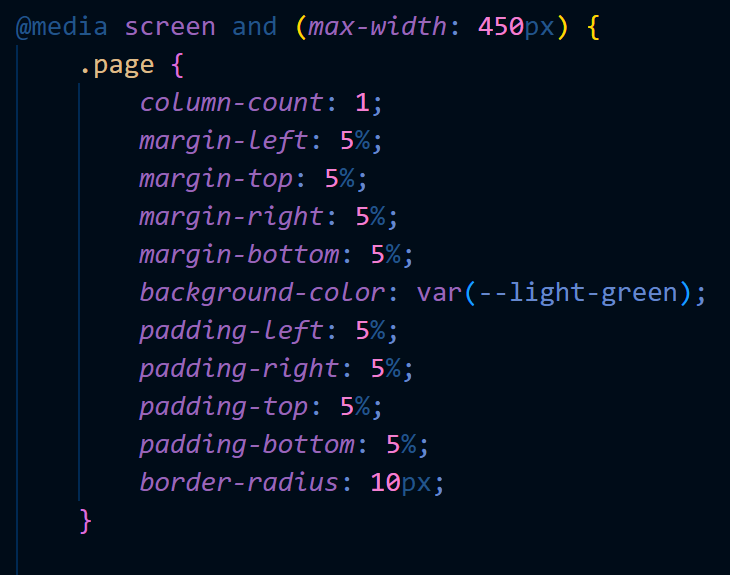
\includegraphics[width = 10cm, height = 5cm]{Photos/mediascreen.PNG}
    \caption{CSS pour un téléphone portable : affichage sur une seule colonne}
    \label{fig:my_label}
\end{figure}
\vspace{5cm}
\newline 
\subsubsection{Page connexion}
Quand les utilisateurs se sont déjà inscrits une première fois, il est nécessaire qu'ils puissent accéder de nouveau à leur profil. En se rendant dans Connexion sur le bandeau déconnecté, ils arriveront sur la page Connexion.
\begin{figure}[h!]
    \centering
    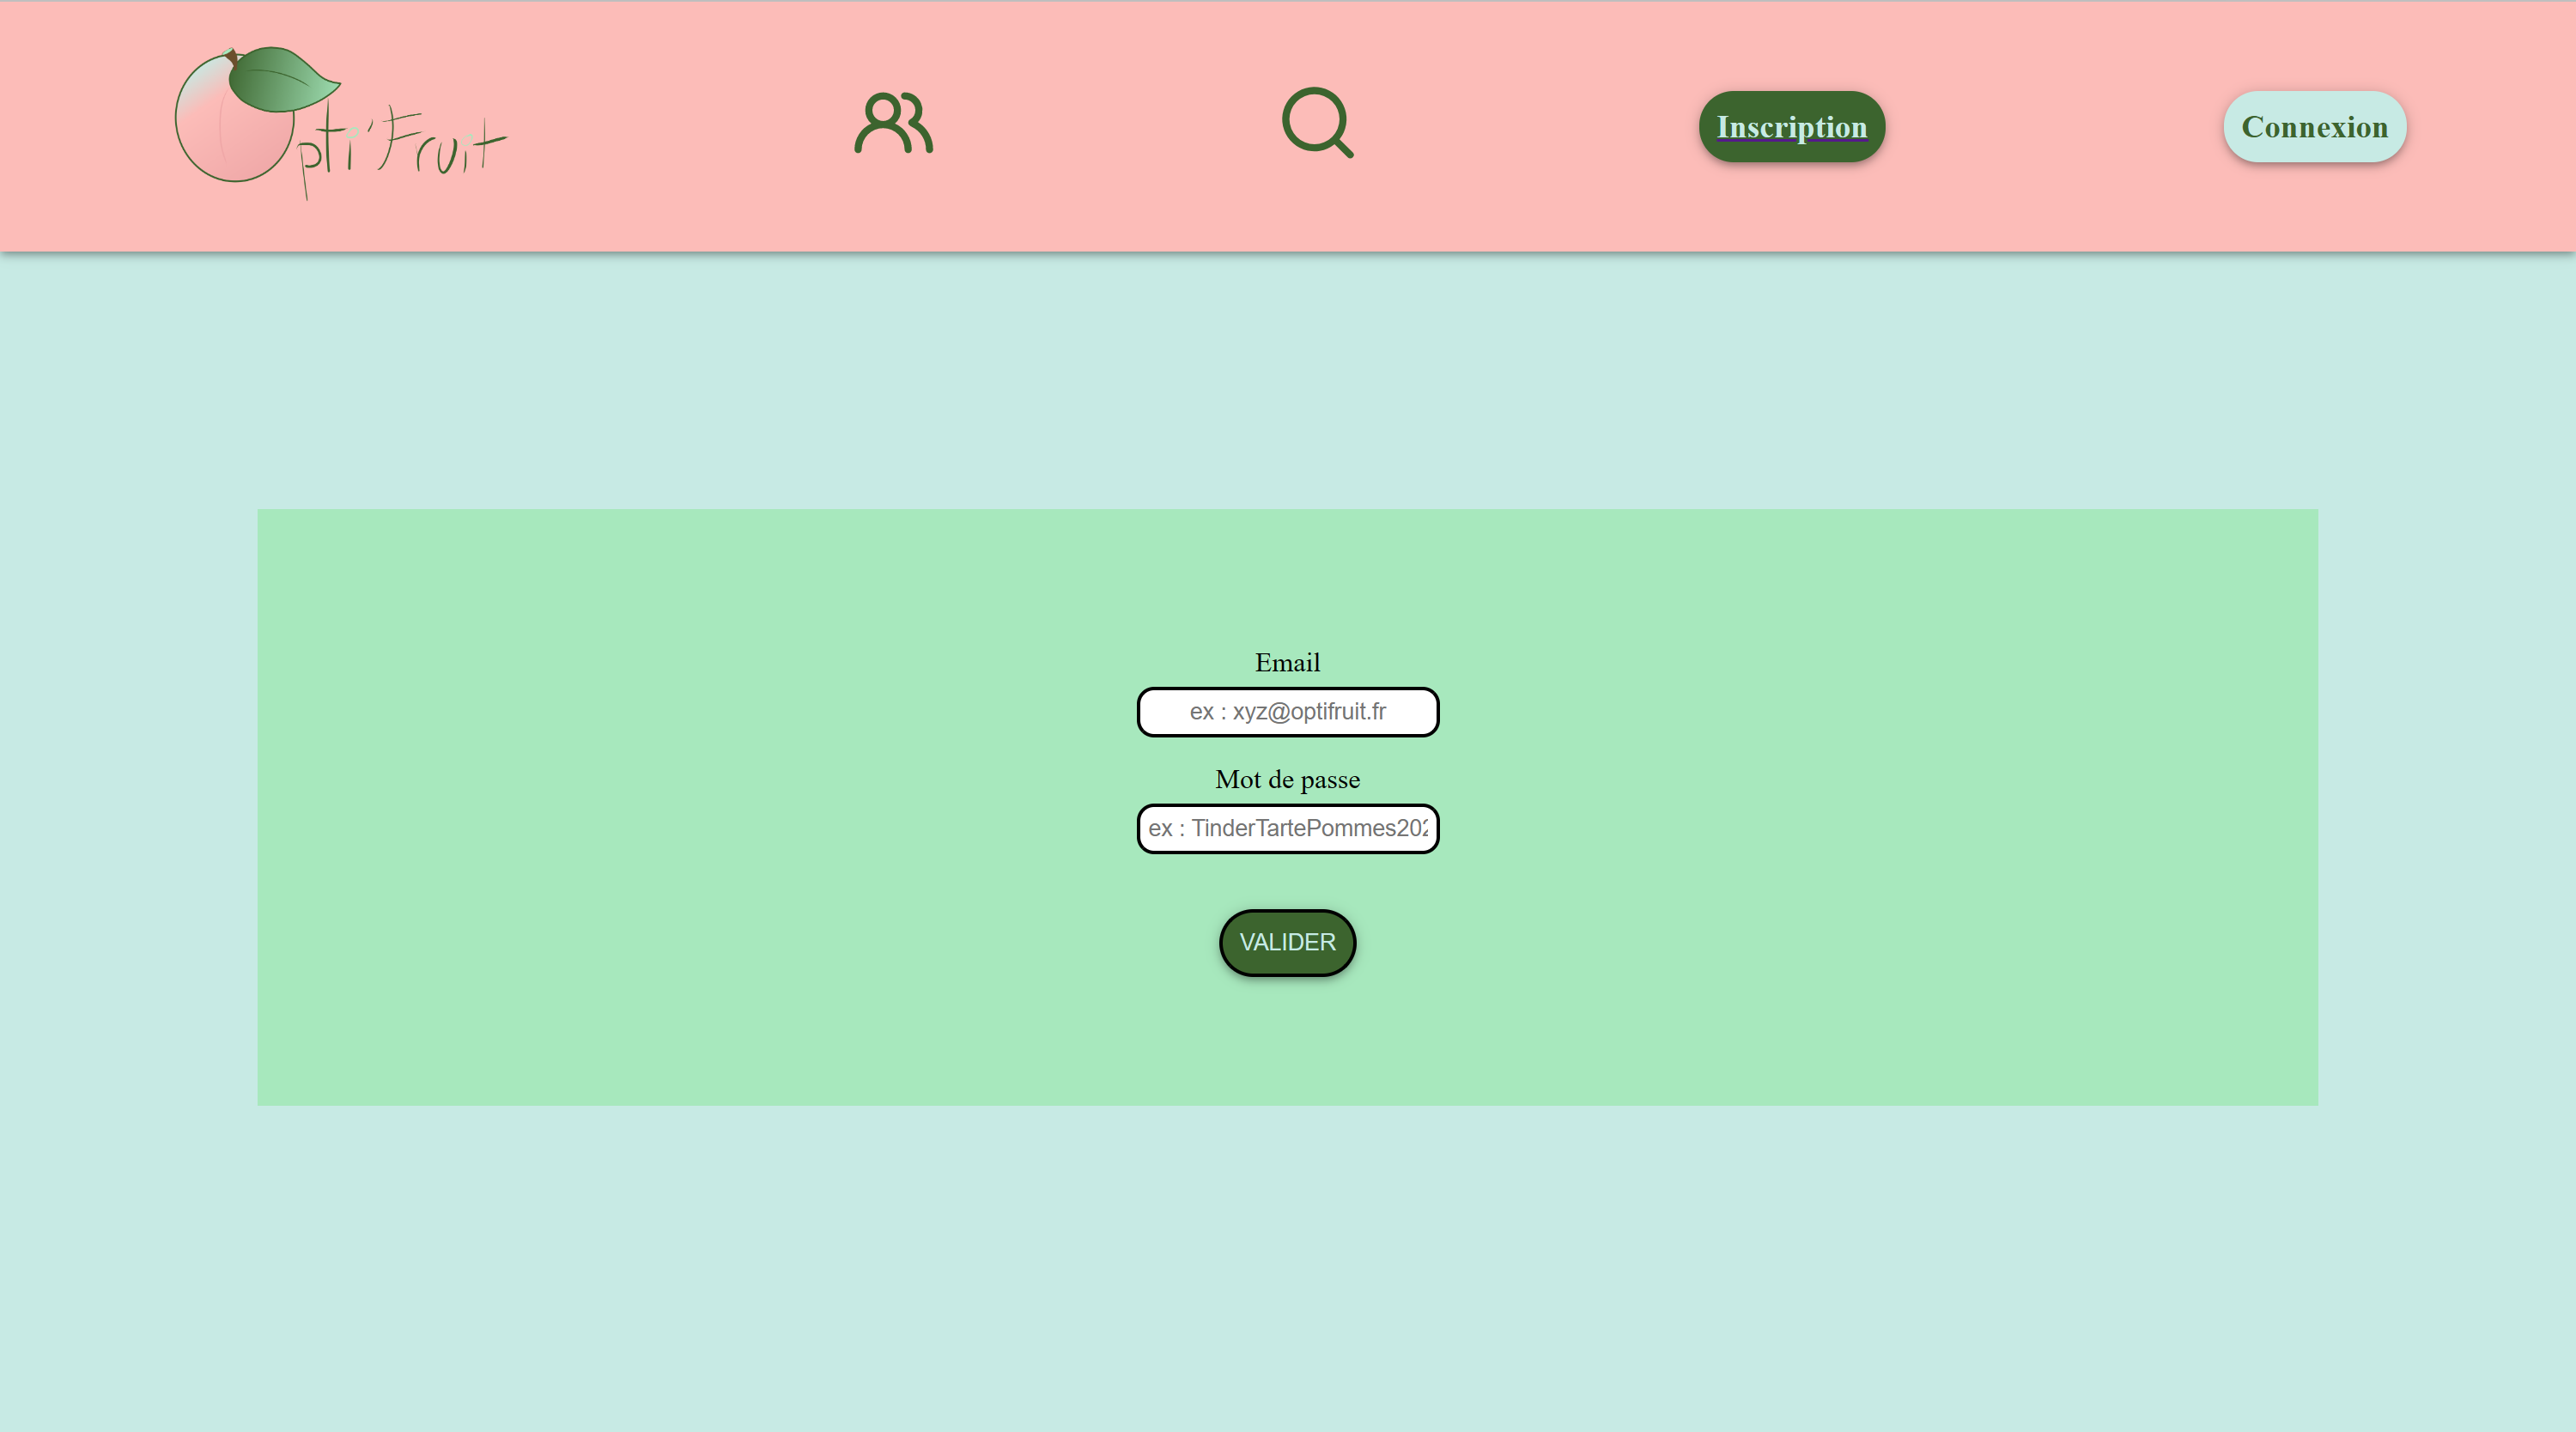
\includegraphics[width = 10cm]{Photos/Connexion.PNG}
    \caption{Page de connexion}
    \label{fig:my_label}
\end{figure} 
\vspace{1cm}
\newline Son \textbf{adresse mail} et son \textbf{mot de passe} sont récupérés à l'aide de request form. Si au moins un des deux champs n'est pas rempli, un render\_template permet de le signaler à l'utilisateur en affichant un message d'erreur explicite. Il s'agit ensuite de vérifier la véracité des informations fournies. La première étape est de crypter le mot de passe avec le même algorithme que celui utilisé à l'inscription. Il faut ensuite récupérer les mots de passe sous le même format pour les comparer. Si les données sont correctes, l'utilisateur est redirigé vers son profil avec sa session activée. Sinon, l'utilisateur est informé d'un problème de cohérence entre les données.
\begin{figure}[h!]
    \centering
    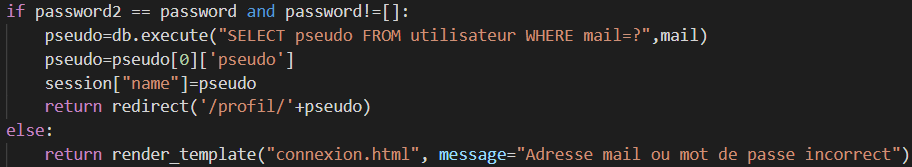
\includegraphics[width = 10cm]{Photos/Checkpassword.PNG}
    \caption{Vérification que le mot de passe correspond à l'adresse renseignée}
    \label{fig:my_label}
\end{figure}
\vspace{5cm}

\subsubsection{Page de profil}
La page de profil regroupe les différentes informations d'un utilisateur auxquelles tout le monde peut y accéder. Les informations sont récupérées à partir du pseudo de l'utilisateur grâce à une requête SQL, les informations affichées sont alors son nom, son prénom, sa photo de profil, ses mentions et ses différentes propositions, qui seront présentées sous la même forme que sur la page d'accueil, en-dessous des informations sur la personne. Si l'utilisateur n'avait pas renseigné de photo de profil, une photo par défaut apparaît. Ensuite, différents boutons apparaissent selon l'utilisateur connecté : si l'utilisateur qui est connecté est le même que celui dont la page de profil s'affiche, il apparaît un bouton \textbf{Se déconnecter}, un bouton \textbf{Supprimer mon compte} et un bouton \textbf{Modifier mes informations}.
\begin{figure}[h!]
    \centering
    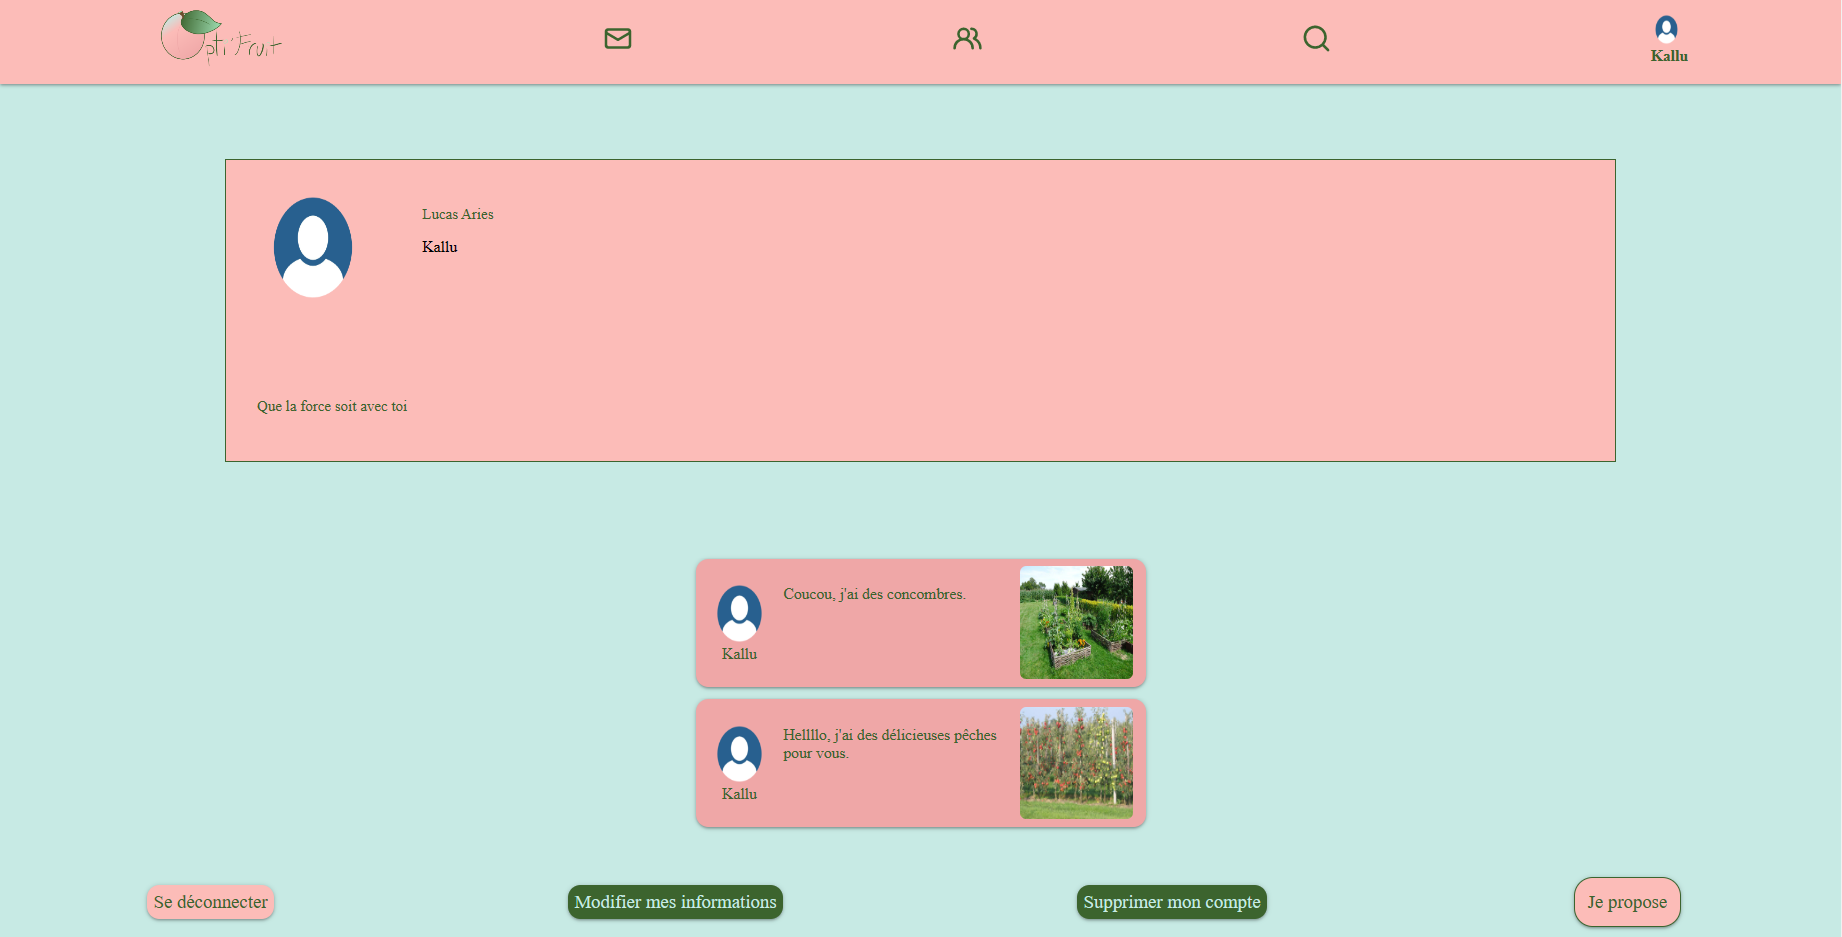
\includegraphics[width = 10cm]{Photos/page profil pareil.png}
    \caption{Page de profil lorsque l'utilisateur connecté est celui du profil affiché}
    \label{fig:my_label}
\end{figure} 
\newline
Le bouton \textbf{Se déconnecter} redirige vers la page \textbf{/logout}, c'est-à-dire vers la page d'accueil tout en déconnectant l'utilisateur. Le bouton \textbf{Supprimer mon compte} supprime l'utlisateur, ses différentes informations, ses propositions et ses messages de la base de données grâce à une requête SQL. Le bouton \textbf{Modifier mes informations} redirige vers la page \textbf{/modifierprofil/pseudo}. 
Si l'utilisateur connecté n'est pas le même que celui dont la page de profil est affichée en revanche, un seul bouton apparaît : \textbf{Envoyer un message à pseudo\_destinataire } qui permet d'envoyer un message à la personne dont le profil est affiché en redirigeant vers la page \textbf{/messagerie/pseudo\_destinataire}.
\begin{figure}[h!]
    \centering
    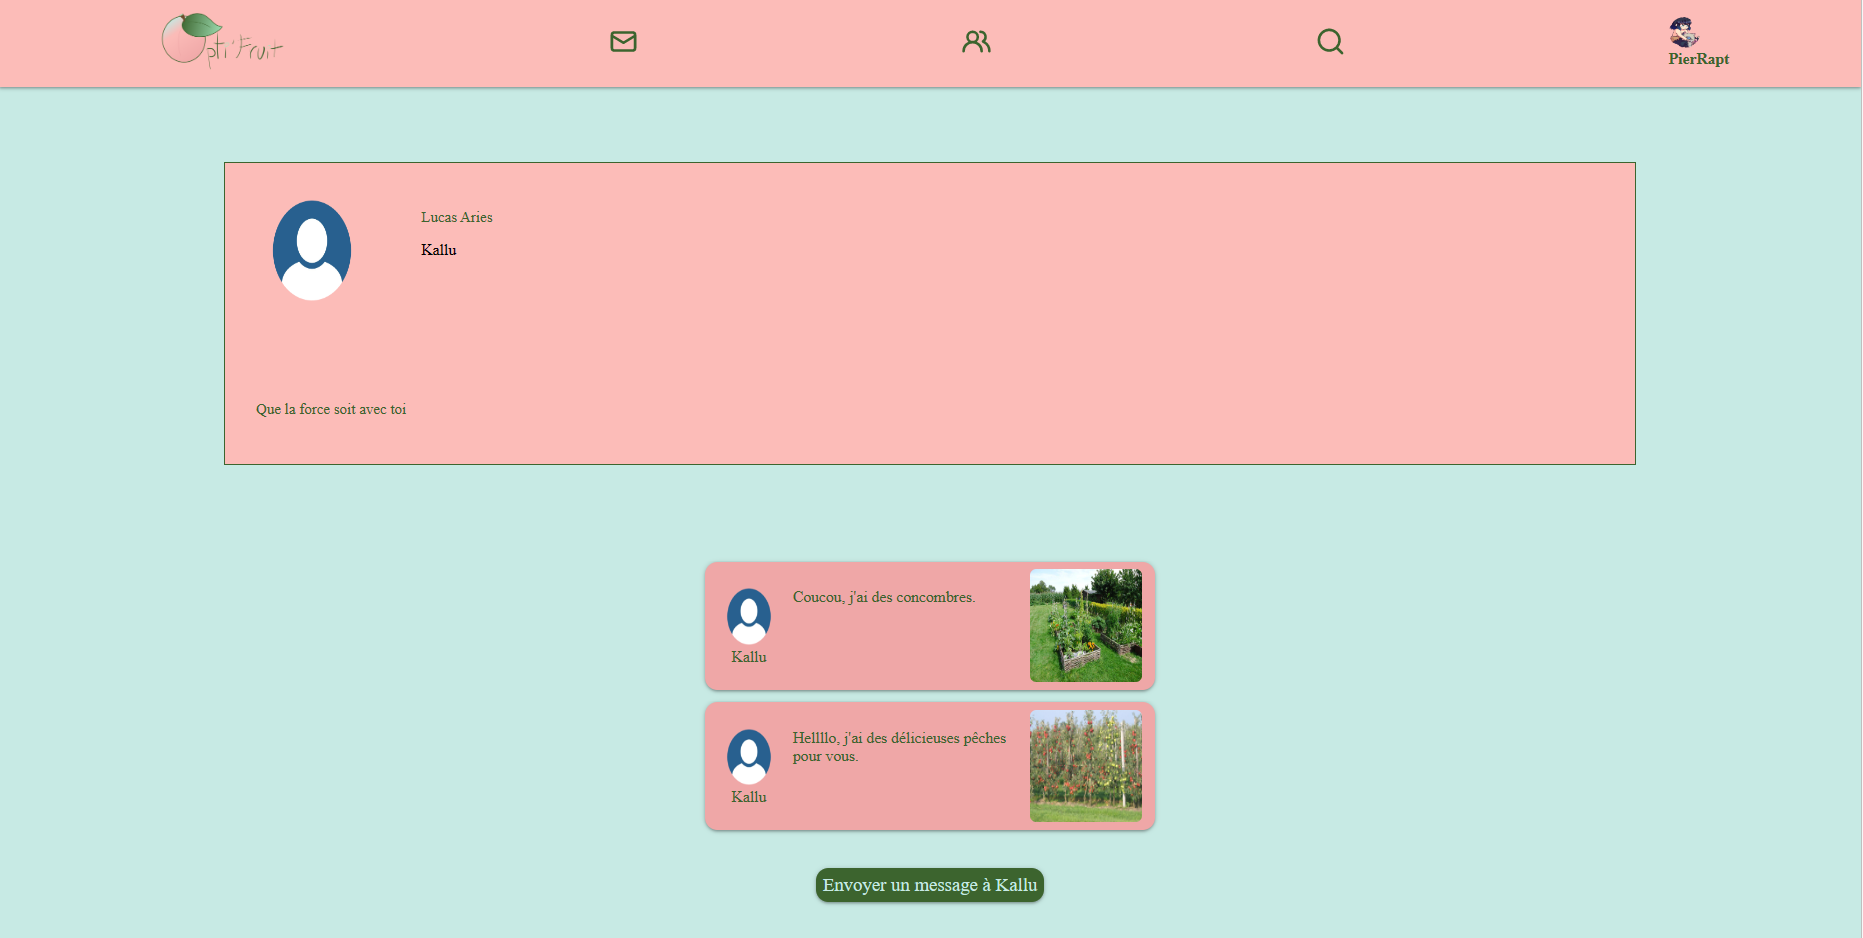
\includegraphics[width = 10cm]{Photos/page profil différents.png}
    \caption{Page de profil lorsque l'utilisateur connecté est différent de celui du profil affiché}
    \label{fig:my_label}
\end{figure} 
\vspace{4cm}
\subsubsection{Page de modification du profil}
Les utilisateurs ont la possibilité de modifier leurs informations grâce à cette page. Ils peuvent modifier les informations qu'ils souhaitent en remplissant uniquement les champs qu'ils souhaitent modifier : leurs \textbf{nom}, \textbf{prénom}, \textbf{pseudo}, \textbf{numéro de téléphone}, \textbf{adressse mail}, une \textbf{mention}, une \textbf{photo de profil} ou leur \textbf{mot de passe} qu'ils devront confirmer. Ce mot de passe devra également contenir entre 8 et 20 caractères pour des raisons de complexité et sa validité sera vérifiée avant son cryptage. Le cryptage permet de ne pas enregistrer le mot de passse brut dans la base de données. Si le mot de passe n'est pas conforme à ces attentes, un message d'erreur adapté sera renvoyé, comme pour la page d'inscription.
Une fois que l'utilisateur a rempli les champs qu'il souhaitait modifier, un clic sur le bouton \textbf{Modifier} activera la méthode \textbf{POST} de la page.
\begin{figure}[h!]
    \centering
    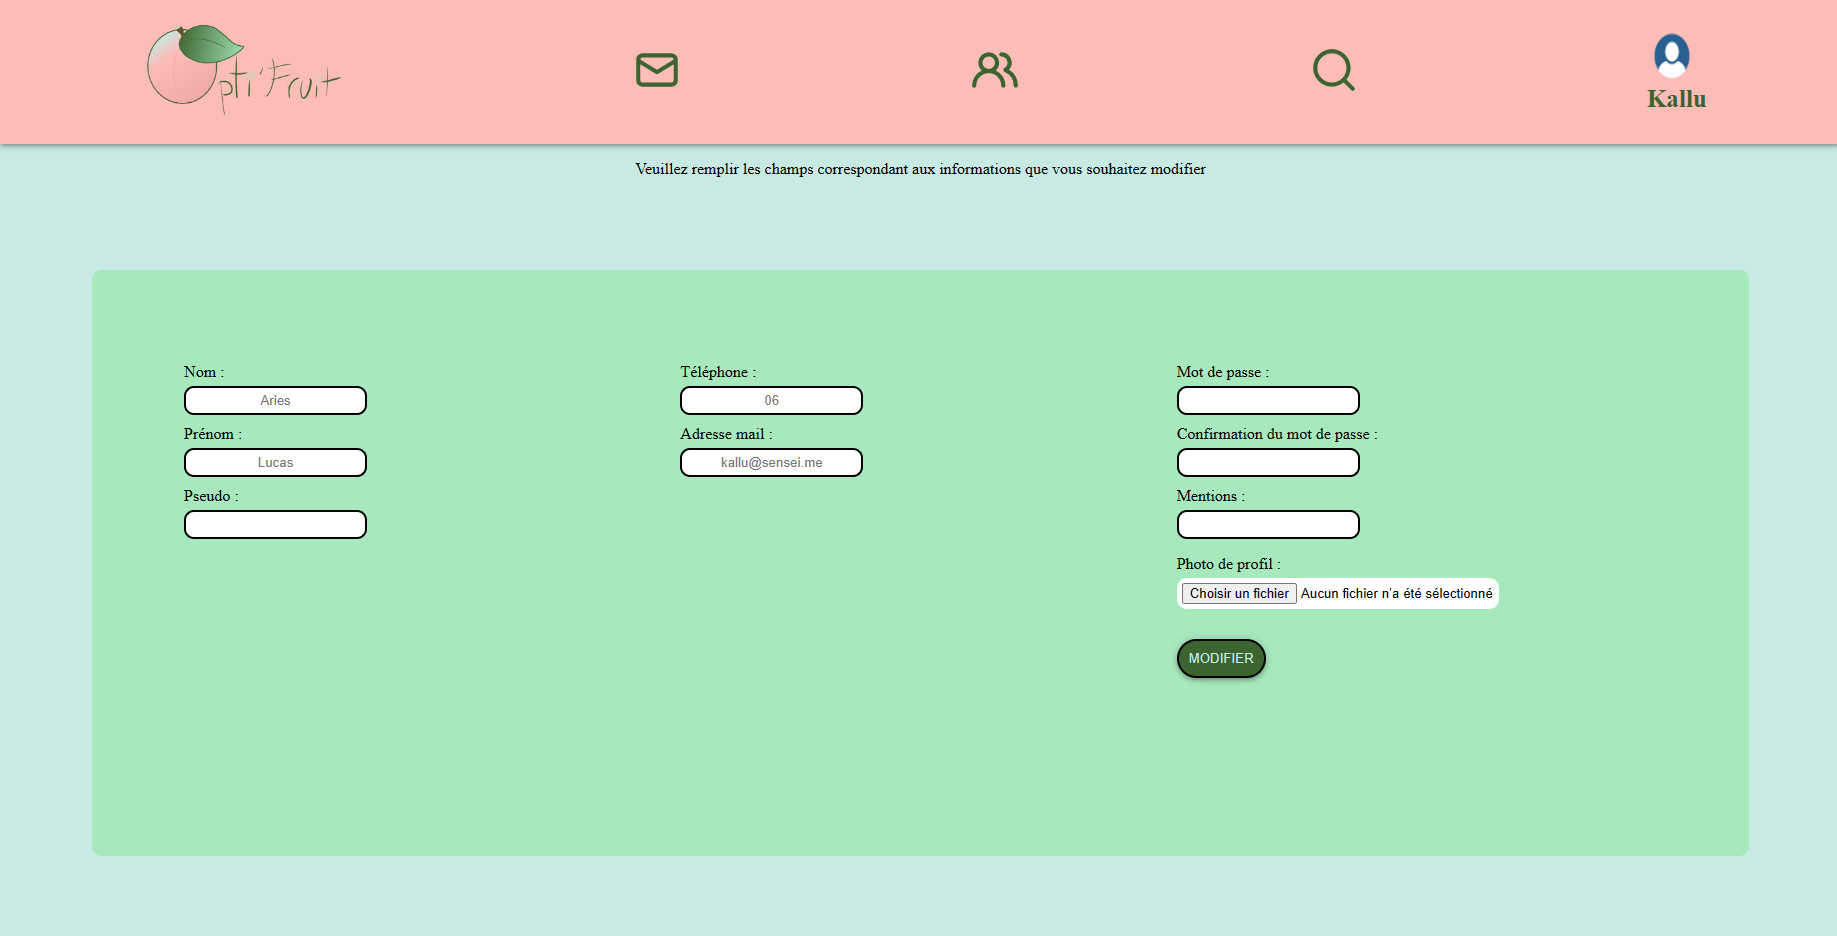
\includegraphics[width = 10cm]{Photos/page modif profil.png}
    \caption{Page de modification du profil}
    \label{fig:my_label}
\end{figure} 
\newline
Les données seront récupérées grâce à des request. Pour chaque information que l'utilisateur a changé, la commande \textbf{UPDATE} pour les requêtes SQL est utilisée. Enfin, si le pseudo fait partie des informations à changer, étant donné qu'il est la clé primaire de la table \textbf{utilisateur} et une clé étrangère des tables \textbf{proposition} et \textbf{messagerie} plusieurs requêtes SQL doivent être faites. Il faut insérer le nouveau tuple correspondant dans la table \textbf{utilisateur} en récupérant au préalable toutes les autres informations dans la table concernant cet utilisateur, faire les modifications nécessaires dans les tables \textbf{proposition} et \textbf{messagerie} et enfin supprimer le tuple avec l'ancien pseudo dans la table \textbf{utilisateur}.
\begin{figure}[h!]
    \centering
    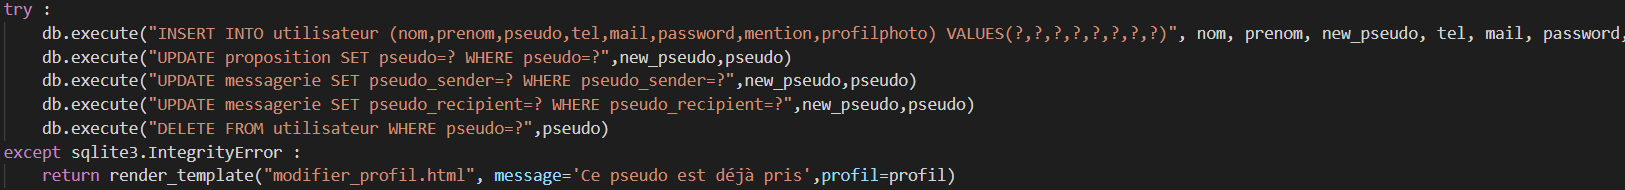
\includegraphics[width = 10cm]{Photos/requetes sql modif profil.png}
    \caption{Différentes requêtes SQL}
    \label{fig:my_label}
\end{figure}
\newline
L'utilisateur est ensuite redirigé vers la page \textbf{profil}.


\subsubsection{Page recherche}
Cette page permet à chaque utilisateur d'effectuer des recherches de fruits et légumes selon plusieurs critères: le code postal, le département et la région. Les deux premiers critères de recherches permettent de trouver des résultats à proximité et sont ainsi représentatifs de circuits courts. Le critère de recherche par région est moins pertinent, mais permet à chacun d'avoir une vision d'ensemble de ce qui est proposé sur l'application, et semble ainsi pertinente pour les nouveaux utilisateurs ou ceux qui hésiteraient encore à se servir de l'application et qui souhaiteraient simplement voir ce qui peut se trouver dessus.
Les résultats sont \textbf{ORDER BY} par code postal, quelque soit le critère de recherche.

\subsection{Algorithmes de traitement}
        \subsubsection{Suppression d'une proposition quand la date est dépassée}

Afin de ne pas surcharger l'application avec des propositions dépassées, un algorithme supprime automatiquement ces propositions à l'ouverture de l'application.

Pour cela, nous avons créé une fonction \textbf{pastPropositions}, ne prenant pas d'argument d'entrée, et ne renvoyant rien. Cette fonction récupère la date actuelle, et, sous forme de liste, les identifiants et les dates d'expiration de toutes les propositions existantes. Ensuite, la fonction compare l'année de fin de la proposition avec l'année actuelle. Si elle est plus petite, la fonction supprime dans la base de donnée la proposition portant le même identifiant. Sinon, si elles sont égales, elle fait les mêmes tests pour le mois, puis le jour.

La complexité de cet algorithme est linéaire.

        \subsubsection{Vérification de l'extension des fichiers}
Lors de l'inscription ou lors de l'ajout d'une proposition, on a la possibilité d'ajouter une photo. Dans les deux cas, il faut bien s'assurer que les fichiers récupérés soient bien des images.

Pour cela, la fonction \textbf{allowed\_file} récupère le nom du fichier et renvoie un booléen caractérisant si l'extention du fichier est dans la liste \textbf{allowed\_extention}, définie au préalable. Cette dernière est la liste des extentions voulues. La fonction va séparer le nom donné en paramètre en plusieurs chaînes de caractères, à chaque apparition du caractère \textbf{.} ,  avec la fonction \textbf{split}. On aura donc une liste de chaque partie du nom ainsi séparé. Si le nom est un nom de fichier valide, la liste doit être de longueur 2, composée du nom donné par l'utilisateur, et de son extension. Si ce n'est pas le cas, la fonction renvoie \textbf{False}. Sinon, elle teste si l'extension est dans la liste \textbf{allowed\_extention}, et renvoie le résultat de ce test.

La complexité de cet algorithme est linéaire.

\newpage
\subsubsection{Cryptage du mot de passe}
Lors de l'inscription ou de la modification du mot de passe d'un utilisateur, ce mot de passe doit être crypté pour des raisons de sécurité. L'algorithme prend en argument notre mot de passe sous forme de chaînes de caractères, le transforme ensuite en liste de caractères et crée une liste de la même taille que notre mot de passe contenant uniquement des 0 qui représentera par la suite le mot de passe crypté. 

À l'aide d'une fonction auxiliaire récursive, on va ensuite crypter notre mot de passe, cette fonction va prendre en argument le mot de passe à crypter sous forme de liste et l'indice de la liste donnant la position du caractère à crypter dans notre mot de passe. La fonction prend chaque élément de la liste (donc chaque caractère du mot de passe) et le cherche dans une liste contenant les caractères ASCII : la recherche démarre au premier élément de la liste ASCII et s'arrête lorsque le caractère est trouvé. Tant que le caractère n'est pas trouvé, chaque élément de la liste représentant notre mot de passe crypté, à partir de l'indice pris en argument (qui correspond au caractère actuellement étudié du mot de passe) est incrémenté de 1. Ensuite la fonction auxiliare est réappliquée à la liste représentant le mot de passe privée de l'élément qui vient d'être étudié et à l'indice de la liste donnant la position du caractère à crypter, c'est-à-dire le précédent indice incrémenté de 1. 

Lorsque la liste représentant le mot de passe à crypter donnée en argument à la fonction récursive est vide (qu'il n'y a plus de caractère à crypter), la liste de chiffres représentant le mot de passe crypté est alors changée en une liste de caractères en remplaçant chaque nombre par l'élément correspondant dans la liste ASCII (si le nombre est plus grand que la longueur de la liste ASCII, il est décrémenté de cette même longueur jusqu'à arriver à un nombre compris entre 0 et la longueur de la liste ASCII). Cette liste de caractères est alors changée en une chaîne de caractères pour obtenir le mot de passe crypté.

La complexité de cet algorithme est quadratique.

\newpage
\section{Tests et performances}
\subsection{Suppression d'une proposition quand la date est dépassée}
Un ensemble de tests a été réalisé, dans un fichier \textbf{test\_pastPropose.py}, invocable par pytest. Tout d'abord, nous testons différentes valeurs pour le jour, le mois et l'année de la date (plus petite, égale ou plus grande que la date actuelle). Ensuite, on teste si l'un des trois n'est pas un entier, ou s'il est manquant, et si la date est bien du bon format. Puis, on teste si la date est vide, s'il n'y a pas de date ou s'il n'y a pas de proposition. Enfin, on teste pour deux propositions, lorsque les deux sont dépassées, et lorsque seulement l'une des deux est dépassée.

\subsection{Vérification de l'extension des fichiers}
Un ensemble de tests a été réalisé, dans un fichier \textbf{test\_allowedFile.py}, invocable par pytest. Les tests considérés sont les suivants : avec un nom de fichier avec chacune des bonnes extensions, avec un nom de fichier avec une extension non valide, avec seulement un nom de fichier sans extension, avec un nom de fichier et un point, avec une extension valide mais un point dans le nom du fichier, avec une chaîne de caractères aléatoires, avec un nom de fichier vide, avec la chaîne vide, avec un entier et avec une chaîne de caractères très longue.

\subsection{Cryptage du mot de passe}
L'algorithme de cryptage du mot de passe est l'algorithme le plus complexe de ce projet. Une estimation manuelle de sa complexité nous a conduit à un résultat en $O(n^2)$, de par la présence de la boucle for imbriquée dans la boucle while. Nous avons par la suite souhaité vérifier ce postulat. Cette vérification se situe dans le fichier \textbf{test\_crypte\_mdp.py}. Nous avons pour cela créé une fonction \textit{timer} qui permet de mesurer le temps d'exécution de l'algorithme pour des valeurs croissantes de longueurs de mots de passe, puis d'en tracer la courbe. Les longueurs choisies varient de 1 à 1000 caractères avec un pas de 50.
La figure suivante illustre ce comportement quadratique

\begin{figure}[h!]
    \centering
    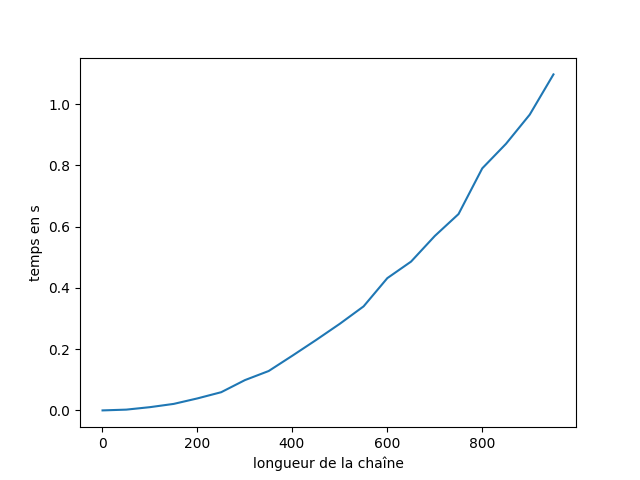
\includegraphics[width = 10cm]{Photos/Figure_1.png}
    \caption{Temps d'exécution en fonction de la longueur de la chaîne}
    \label{fig:my_label}
\end{figure} 

\vspace{6cm}

Le cryptage du mot de passe se réalise à l'aide de deux algorithmes. Le premier \textit{mdpcorrect} permet de vérifier le format du mot de passe. Les tests réalisés sur cet algorithme sont présents dans le fichier \textbf{test\_mdpcorrect.py}. Ces tests se portent sur l'examen de différentes chaînes de caractères, de tous formats et de toutes natures. Les chaînes de caractères vides mais également les éléments qui ne sont pas des chaînes de caractères sont testés.


Le second algorithme est celui qui crypte le mot de passe avant de l'insérer dans la base de données. Ce second algorithme est bien plus complexe et les tests plus difficiles à déterminer.
Deux tests principaux ont ainsi été effectués. Le premier s'attarde sur la longueur des mots de passes cryptés et cherche à vérifier que cette longueur est bien égale à la longueur du mot de passe initial. Pour cela, il génère des mots de passe aléatoires parmi la table ascii de longueurs différentes (de 1 à 1000 caractères) et réalise le test de longueur. Le second test s'intéresse à l'unicité du mot de passe crypté, vérifiant ainsi que deux mots de passe différents ne puissent être cryptés de la même manière. Le test génère ainsi un nombre important de mots de passe \textbf{différents} et vérifie que la liste contenant les mots de passe cryptés ne contient pas deux fois la même itération d'un mot de passe.

\newpage
\section{Gestion de projet}

\vspace{8mm}
\subsection{Cahier des charges}

\subsubsection{Contexte et description du projet}

\vspace{1cm}
\textbf{Présentation de l'application pour les clients}

Les pommes, c'est bon. C'est encore mieux quand elles viennent de notre jardin. On sait comment elles ont été faites, elles sont bios, locales, et c'est ce qui nous les fait aimer encore plus. Mais quand notre pommier est trop gros, on a trop de pommes, et bien souvent la majorité tombent par terre et ne sont jamais récupérées. De même quand on part en voyage et qu'on ne peut pas les ramasser, elles pourrissent aussi sans qu'on puisse en profiter.

Mais pourquoi ne pas en faire profiter les autres ? Comment trouver un moyen d'avertir les personnes intéressées de notre surplus de fruits ou légumes ? C'est de là que vient l'idée de notre application web : une interface de rencontre et de partage, pour échanger, donner et recevoir des fruits et légumes locaux, et venir en aide à nos voisins.
Facilitant l'accès à des produits bios et locaux, cette application permet aux personnes de vendre ou donner ce qu'ils ont cultivé, ou de rechercher des produits près de chez eux. Pour cela rien de plus simple ; il suffit de s'inscrire, renseigner sa localisation, et spécifier nos besoins. Grâce à une carte interactive, on peut facilement avoir accès à ce que proposent nos voisins.

Envie de vendre, échanger ou donner ses produits ? Besoin d'aide pour les récoltes que l'on ne peut pas effectuer ? Une petite annonce et le tour est joué ! Et en y ajoutant des photos, les autres utilisateurs se feront une meilleure idée. Mais si personne ne veut de mes produits ? Pas de panique, si au bout d'un certain temps personne ne se propose, l'application vous donnera la possibilité de faire don à une association.
Une envie de fruits ou légumes en particulier ? Vous pouvez simplement faire une recherche, et l'application vous retourne les résultats près de chez vous. Quelque soit votre besoin, les propositions tiendront compte de la distance géographique.
Enfin, lorsque vous trouvez des personnes intéressées, un système de messagerie permet alors d'échanger diverses informations, de discuter, et d'avoir une trace des engagements de chacun.

Ainsi, cette application web permet aux jardins privés de limiter le gaspillage, mais aussi d'échanger avec d'autres personnes qui partagent vos envies.
\vspace{1cm}
\newline
\textbf{Présentation et description technique de l'application}

Notre projet consiste en une application web permettant de vendre et d'échanger ses fruits et légumes, tout en proposant des cueillettes directement chez le particulier. Pour cela, il y aura possibilité de déposer des annonces de vente de fruits et légumes, de troc ou encore de cueillette. 

Chaque particulier pourra alors rechercher le produit qu'il désire parmi ces annonces proches de chez lui. En effet, une carte interactive permettra de voir la localisation des différents produits, cette localisation ne sera pas précise mais donnée par zone géographique. Les produits seront proposés dans un périmètre donné autour de la localisation du client, périmètre qui augmentera au fil du temps, dans un objectif de limiter la consommation de carburant provoquée par de longs trajets et donc la pollution atmosphérique. 

Un système de messagerie permettra de mettre en contact la personne intéressée et la personne proposant le produit, afin qu'elles puissent convenir d'une date et d'un lieu de rendez-vous. 
La problématique des cambriolages s'est posée lors de la réflexion sur le système de cueillette, cependant chaque particulier ne donnera sa localisation précise uniquement s'il le souhaite via la messagerie et décidera seul s'il accepte qu'une autre personne vienne chez lui sans sa présence. De plus, les cueillettes peuvent également se faire lorsque la personne est présente, par exemple lors d'une journée de télé-travail.

Dans les derniers jours de consommation du produit, s'il n'a pas pu être vendu ou échangé, il sera proposé à l'utilisateur d'en faire don à une association. 

\subsubsection{Objectif et périmètre du projet}

Nous souhaitons ainsi offrir à nos utilisateurs un service plus complet que ceux existant actuellement. Une application qui leur permet de gérer leurs surplus, mais également d'aider à la récolte même, un élément souvent oublié lorsque l'on parle de gaspillage.
Pour cela, nous nous concentrerons sur tout le territoire français.

\subsubsection{Description fonctionnelle des besoins}

\begin{tabular}{|p{3.5cm}|p {3.5cm}|c|c|c|} \hline
    Fonction & Objectif & Degré de liberté & Niveau de priorité  \\ \hline
    Permettre à l'utilisateur de proposer ses fruits  & Saisir facilement ses informations & Faible & Élevé \\ \hline
    Accéder à l'ensemble des informations via une carte interactive & Permettre à l'utilisateur de s'y retrouver facilement & Moyen & Moyen \\ \hline
    Permettre aux utilisateurs de se contacter via l'application & Faciliter les échanges entre utilisateurs & Élevé & Moyen \\ \hline
    Renvoyer vers une association & Ne pas gaspiller alors que des solutions existent & Faible & Élevé \\ \hline
\end{tabular}


\subsubsection{Enveloppe budgétaire et ressources disponibles}

Ce projet n'a pas de budget alloué. L'équipe projet est composée de 4 membres qui travailleront directement avec leurs matériels personnels ou celui de l'établissement.

\subsubsection{Délais}

Le projet se décompose en différents livrables et différentes échéances:
\begin{itemize}
    \item Le premier livrable se compose d'un rapport à déposer avant le 20/10/2022.
    \item Le second livrable correspond au rendu du projet. Ce dernier a lieu le 11/01/2023.
\end{itemize}

\vspace{8 mm}



\subsection{Charte Projet}

\subsubsection{Contexte}

Aujourd'hui, les circuits courts sont les alternatives les plus intéressantes face au défi qu'est devenu la gestion de l'alimentation et de l'eau. De nombreuses solutions sont apparues pour faire face à ce défi. On peut retrouver les jardins partagés, les micro-fermes mais également le partage de ressources produites au sein de jardins privés. 

Ces applications sont principalement utilisées par les propriétaires de jardin privés. Chacune d'entre elles permet de répondre à sa manière à la problématique du surplus de production dans ces jardins ainsi que leur gestion.

Le cahier des charges permet d'identifier de manière immédiate les principaux besoins et fonctions auxquels l'application doit répondre. Il s'agit notamment de permettre de mettre en relation des propriétaires de jardins privés, de permettre de gérer le surplus de production mais également de permettre une meilleure gestion de la récolte afin d'éviter les pertes initiales.


\subsubsection{Finalités et importance du projet: Business Case}

Ce projet est aujourd'hui essentiel afin de répondre aux problématiques actuelles concernant la gestion de l'alimentation en circuits courts. De plus, la nature même du projet et ses coûts extrêmements limités réduisent la néceesité d'un retour sur investissement, permettant ainsi un départ peu risqué. L'application visant à proposer un service sans recherche de bénéfices, l'estimation de ces derniers est inutile.

De manière prévisionnelle, on peut estimer que l'application permettra de mettre en relation de nombreux propriétaires de jardins privés au sein de communes principalement en zone rurale. Sa gestion des récoltes participera à une nouvelle manière de partager des surplus de fruits non consommés, une innovation qui permettra une ouverture plus grande que la plupart des projets existants.

\vspace{4mm}

Les parties prenantes relatives au projets sont: l'équipe projet, composée de quatre membres, les enseignants encadrants, ainsi que les potentiels utilisateurs de l'application.

Le périmètre du projet s'étend sur tout le territoire français, mais la nature même de son fonctionnement favorise une utilisation dans des zones rurales où le nombre de jardins privés est bien plus important.
A cette limite géographique s'ajoutent de nombreux prérequis à obtenir: obtention des compétences nécessaires au développement d'une application web et de la création d'algorithme, être dans un cadre légal quant à la possibilité de venir récolter les fruits chez une autre personne.

\vspace{4mm}
 
Cette analyse du Business Case permet de proposer une matrice SWOT identifiant les forces, faiblesses, opportunités ainsi que menaces du projet.

\vspace{2mm}             
  
\begin{figure}[h!]
\centering
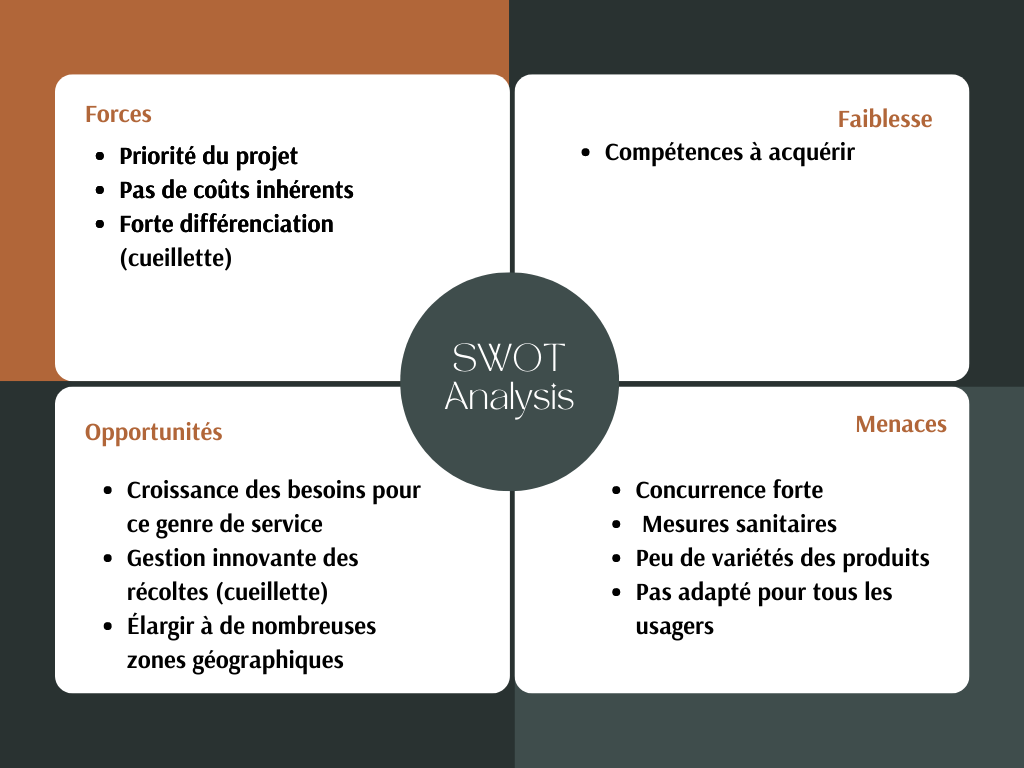
\includegraphics[width = 12cm, height = 9 cm]{Photos/SWOTF.png}
\caption{SWOT relatif à la réalisation du projet}
\label{fig:my_label}
\end{figure}

\newline 
En plus de ce SWOT relatif aux contraintes de réalisation, il est possible d'analyser les forces, faiblesses, opportunités et menaces pour l'équipe et le cadre du projet. 
\begin{figure}[h!]
    \centering
    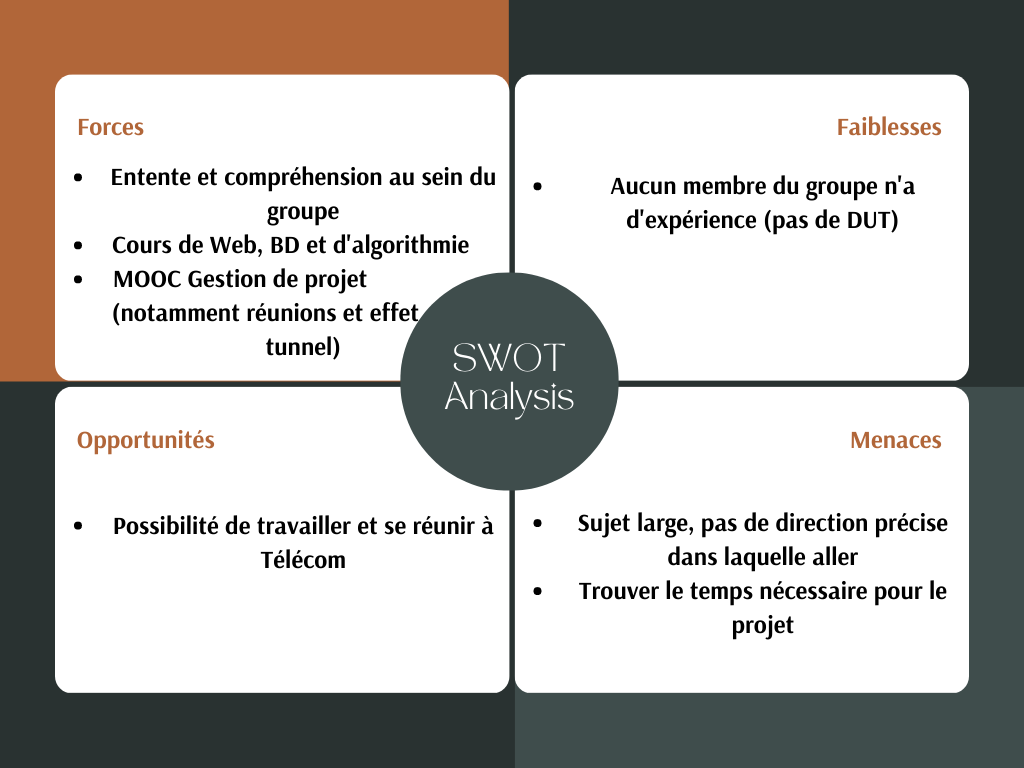
\includegraphics[width = 12cm, height = 9cm]{Photos/SWOT_équipe_projet_uniformisé.png}
    \caption{SWOT relatif à l'équipe et aux consignes}
    \label{fig:my_label}
\end{figure}

\newline
Le manque d'expérience peut être limité par l'exploitation de toutes les ressouces du cours et par un approfondissement sur les documentations officielles des langages utilisés, internet ou en demandant conseil.
L'état de l'art permet également de recentrer les sujets et de nous montrer les principales fonctions déjà existantes. 
De plus, la possibilité de travailler à Télécom pour faire des réunions ou travailler à plusieurs sur un sujet délicat est un gain de temps précieux.

\vspace{1cm}
\maketitle
\subsubsection{Objectifs et résultats opérationnels}

Ces applications connaissent un franc succès aujourd'hui, de par la nécessité de faire face au défi du gaspillage alimentaire, ainsi que par le développement des circuits courts. L'innovation ici proposée, concernant la participation à la récolte même des fruits, permet de s'attaquer à l'une des principales causes de perte de ces derniers. Ces différents éléments sont des indicateurs de la possibilité de succès de ce projet.

\subsubsection{Ressources}
Les moyens à mobiliser sont :
PC personnels et/ou de l'école, postgress4SQL, python3 


\subsubsection{Jalons}
\begin{center}
\begin{tabular}{|p{3cm}|p{5cm}|p{2cm}|} 
  \hline
  Jalon & Description & Date \\
  \hline
  Etape 1 : Exigences opérationnelles & Validation de l'idée lors de la soutenance & 22/10/22 \\
  \hline
  Etape 2 : Création de la base de données & Création de la base de données relative aux fruits et légumes disponibles & 20/11/22 \\
  \hline
  Etape 3 : Réalisation de l'interface & Réalisation de l'interface utilisateur & 20/12/22 \\
  \hline
  Etape 4 : Ajout d'une carte & Ajout d'une carte permettant de repérer où se situent les fruits et légumes & 20/12/22 \\
  \hline
  Etape 6 : Réalisation messagerie & 
  Réalisation d'un système de contact entre les utilsateurs (messagerie) pour obtenir plus d'informations sur un produit en vente ou les conditions d'accueil pour une cueillette & 02/01/23 \\
  \hline
\end{tabular}
\end{center}


\subsection{Matrice RACI}
La matrice RACI permet de nous répartir globalement le travail dans le projet. En
effet pour la plupart des sous-lots, on peut identifier un responsable (l’autorité A), ceux
qui réalisent (R), des conseillers (C) et des personnes à informer (I). Nous n’avons pas fait
figurer les I dans la matrice pour ne pas l’encombrer, car nous avons décidé au début du
projet d’un commun accord que nous nous informerions le plus possible les uns les autres sur
l’avancement de toutes les parties.
\begin{figure}
    \centering
    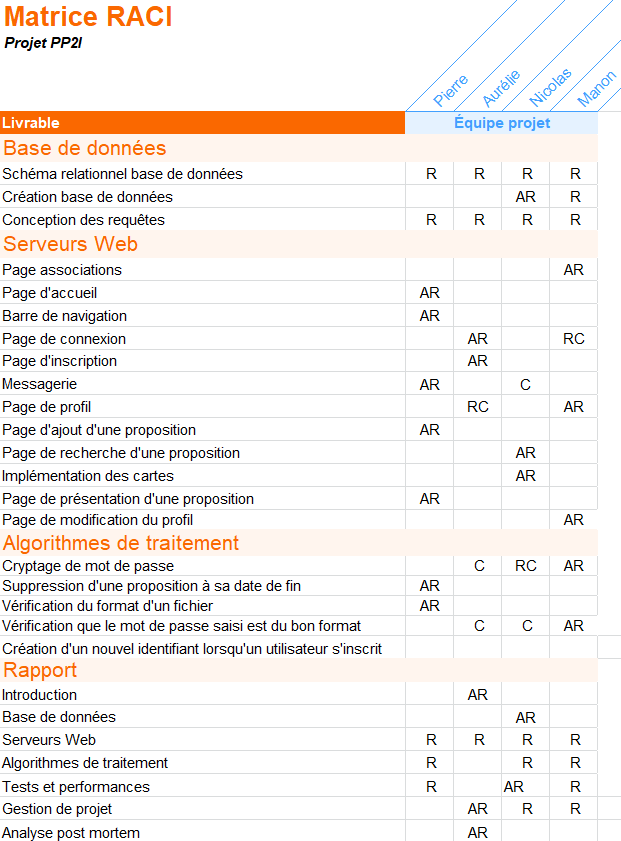
\includegraphics[width = 14cm, height = 12cm]{Photos/matrice_RACI.png}
    \caption{Matrice RACI du projet}
    \label{fig:my_label}
\end{figure}

\newpage
\section{Analyse Post Mortem}
\subsection{Résultats}
Nous avions la volonté de réaliser une application complète avec de nombreuses pages et fonctionnalités. Une bonne partie a été réalisée même si au cours du projet nous avons laissé de côté certaines idées pour approfondir ce que nous avions commencé. Des connaissances d'autres langages tels que le JavaScript auraient pu être utiles mais nous avons su contourner ces difficultés ou ajuster nos idées pour obtenir une application fonctionnelle. 
Cette dernière permet de s'inscrire et se connecter par la suite, de proposer des fruits et des légumes issus de son jardin à d'autres utilisateurs ou de venir récupérer ou cueillir ceux des autres. Les propositions se retrouvent sur la page d'accueil, dans la zone de recherche ou encore sous le profil de celui qui les propose. De plus, vers la date de fin d'une proposition, la page association permet de donner les fruits et légumes avant leur date de péremption. Enfin, les propositions dépassées en date sont automatiquement supprimées.

\subsection{Notions apprises}
    \subsubsection{Gestion de Projet}
    La réalisation d'un état de l'art, la rédaction d'une charte projet, l'analyse de matrices SWOT ou encore la réalisation d'une matrice RACI sont autant d'étapes qui nous ont permis de comprendre le projet, ses enjeux et dangers, et de veiller à répartir et suivre l'avancement des tâches au sein du groupe.
    De plus, les réunions régulières ont évité à des membres du groupe de chercher des solutions seuls trop longtemps ainsi que la création d'un effet tunnel.

    \subsubsection{Base de données, WEB et Algorithmie}
    \begin{itemize}
    \item Nous avons pu créer notre propre base de données après une réflexion collective pour trouver la base optimale. Cette dernière a évolué selon les besoins du projet.
    \item De nombreuses connaissances ont été acquises lors du développement des différentes pages du site aussi bien au niveau du HTML que du CSS selon les fonctionnalités des pages telles que les formulaires ou l'insertion et la récupération de données spécifiques de la base de données.
    \item L'algorithme de cryptage, de suppression des propositions et les autres plus petits algorithmes réalisés nous ont également aidés à nous familiariser avec les méthodes de tests.
   \end{itemize}

\subsection{Points à améliorer}
Pour notre prochain projet, nous consacrerons moins de temps à la maquette que nous avions réalisé pour investir ce temps dans la réalisation du projet même. De plus, il n'est pas nécessaire d'être trop ambitieux, notre objectif est d'avoir un travail réalisant les fonctionnalités qui nous paraissent essentielles sans chercher à multiplier les possibilités du site.
\end{document}
